\chapter{Diseño}\label{cap:diseño}

Este apartado será una descripción de la interfaz gráfica del sistema, reseñando las decisiones tomadas y explicando la navegabilidad.

\section{Inicio de sesión}

En el inicio de la aplicación es donde el usuario inicia sesión con su cuenta si ya está registrado, un acceso para poder ver la actividad donde podrá registrarse y otro acceso que crea un pop-up con el que podremos restablecer la contraseña del usuario en el caso de que haya sido olvidada.

Esta actividad se compone de bloques de textos para el correo electrónico y la contraseña del usuario, un botón para iniciar sesión con esas credenciales y los dos accesos mencionados anteriormente.

\begin{figure}[H]
    \centering
    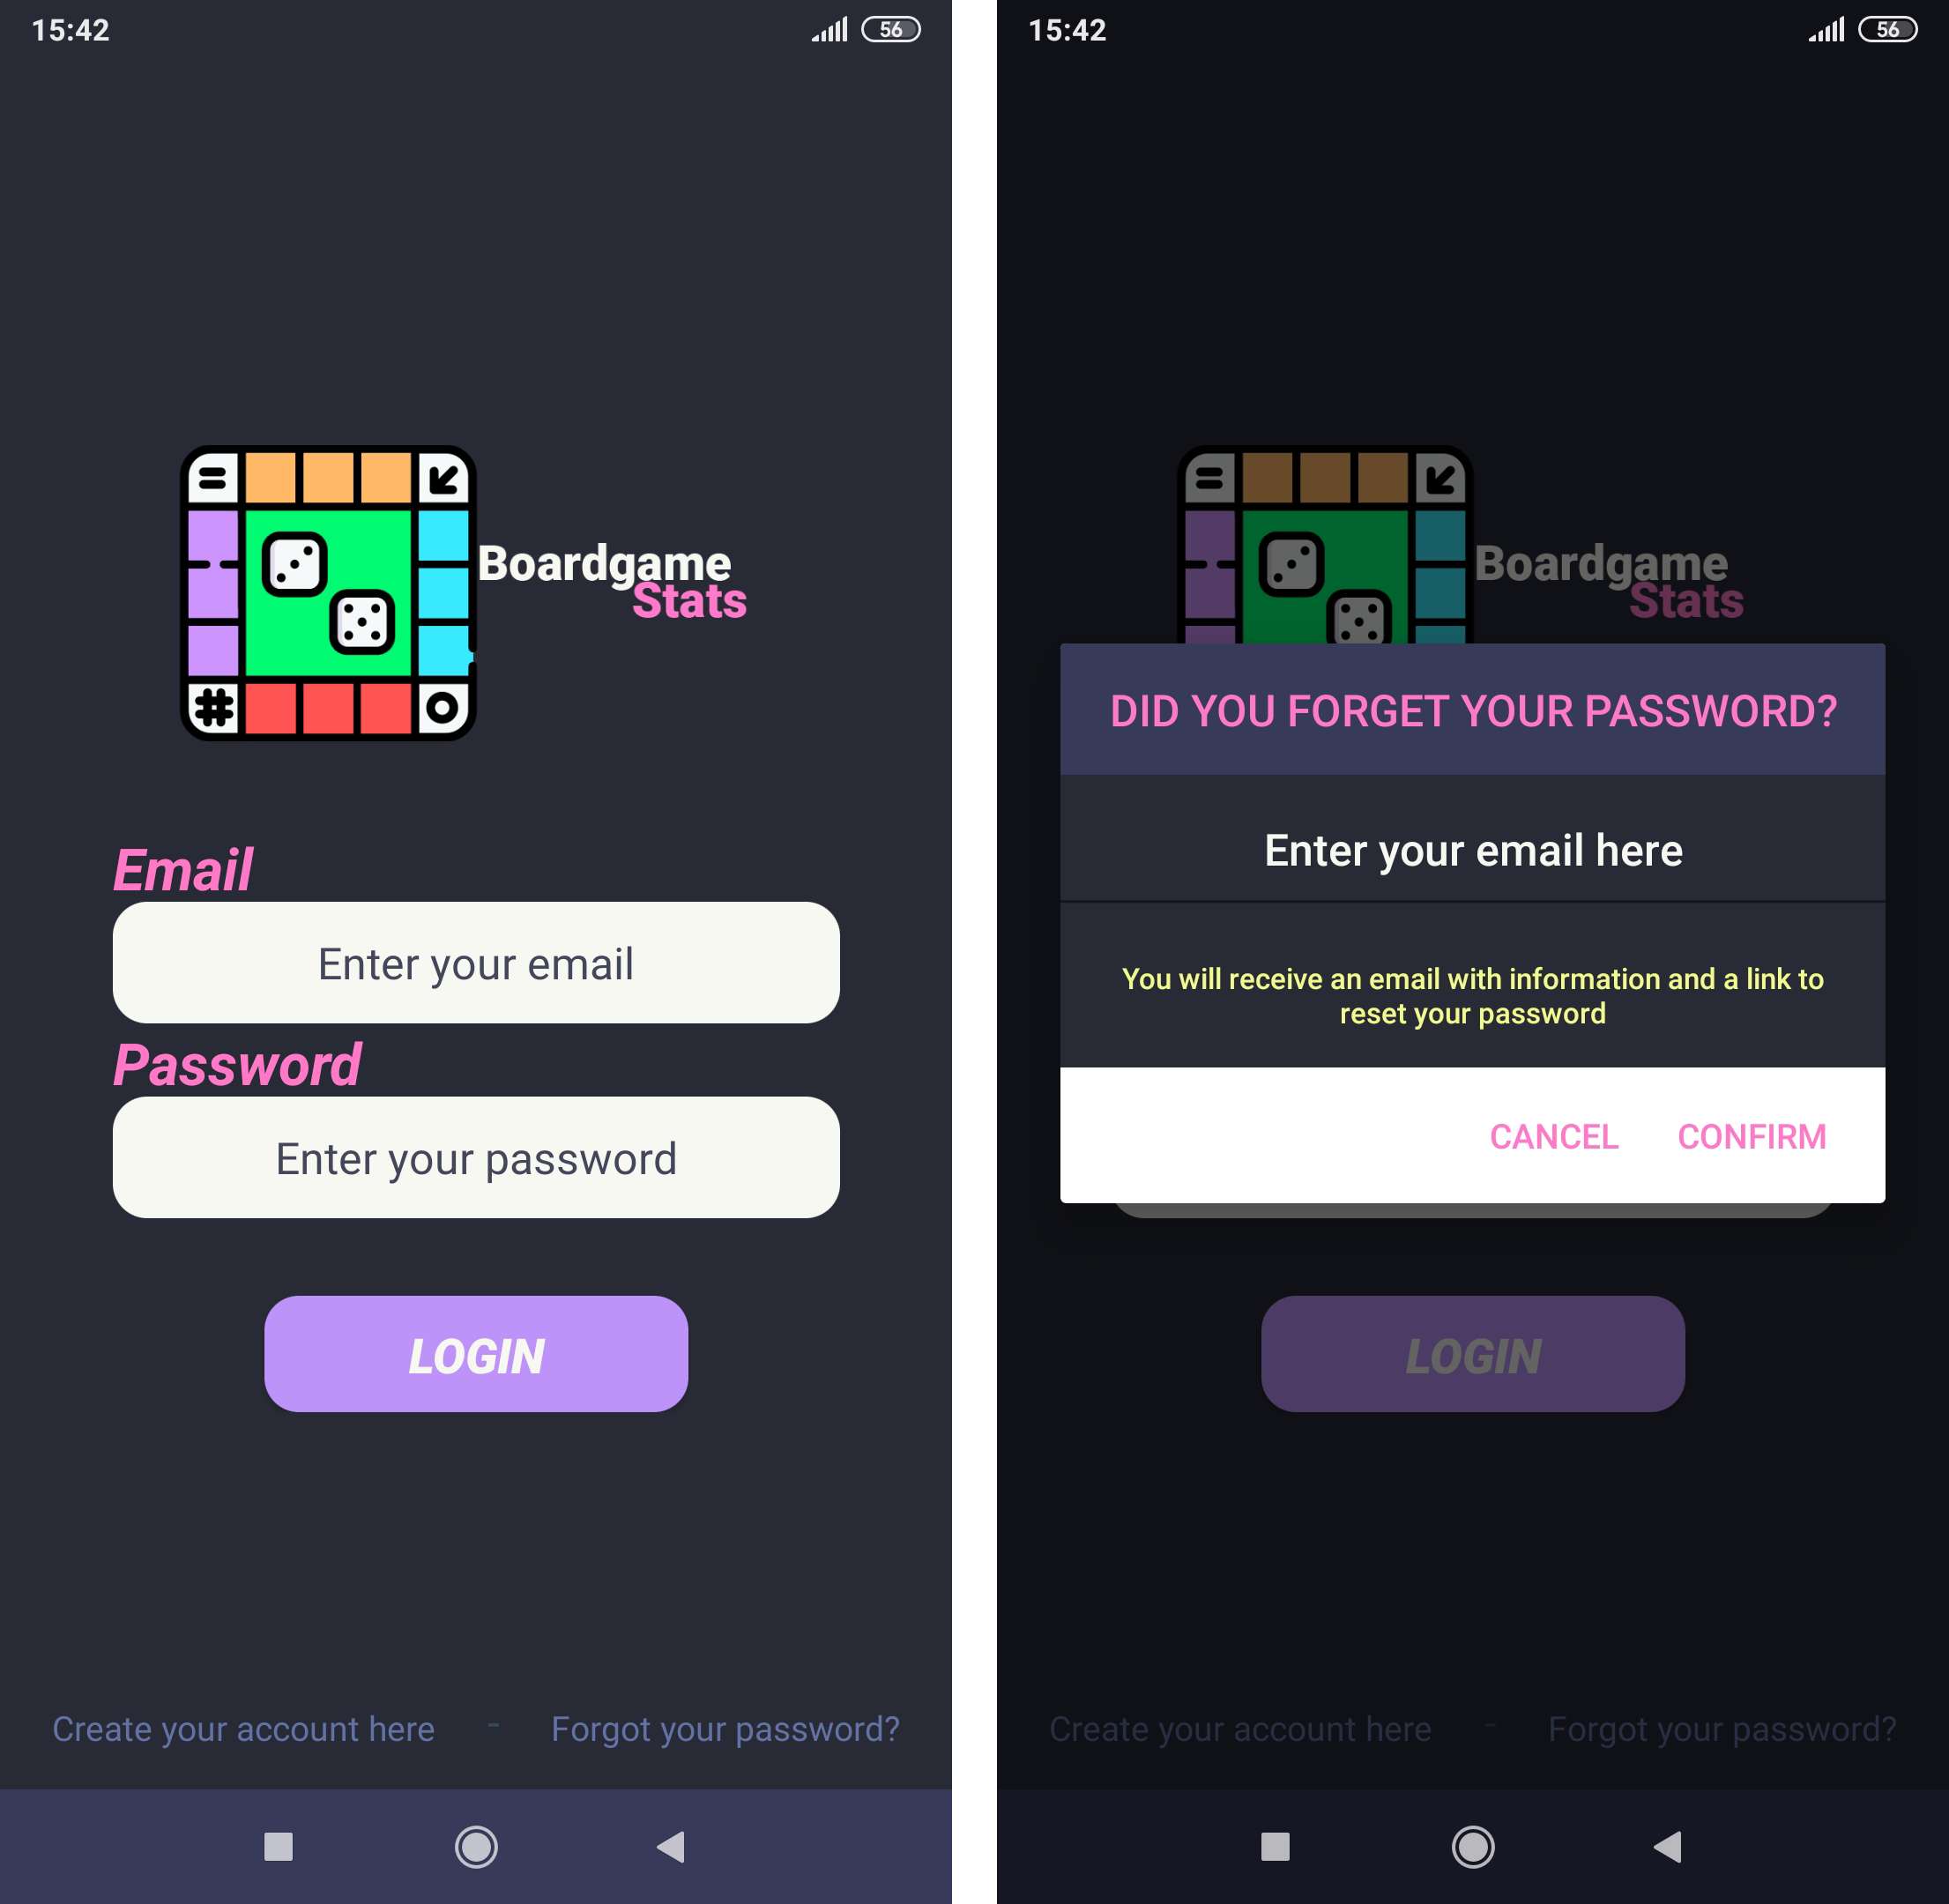
\includegraphics[width=1\linewidth]{fig/Capturas de pantalla de la aplicación/inicio de sesion.png}
    \caption{Inicio de sesión}
    \label{fig:inicio sesion}
\end{figure}

\section{Registro de usuario}

En la actividad de registro nos encontraremos una actividad muy similar a la de inicio de sesión con un leve cambio en el icono y sin los dos accesos anteriores.

\begin{figure}[H]
    \centering
    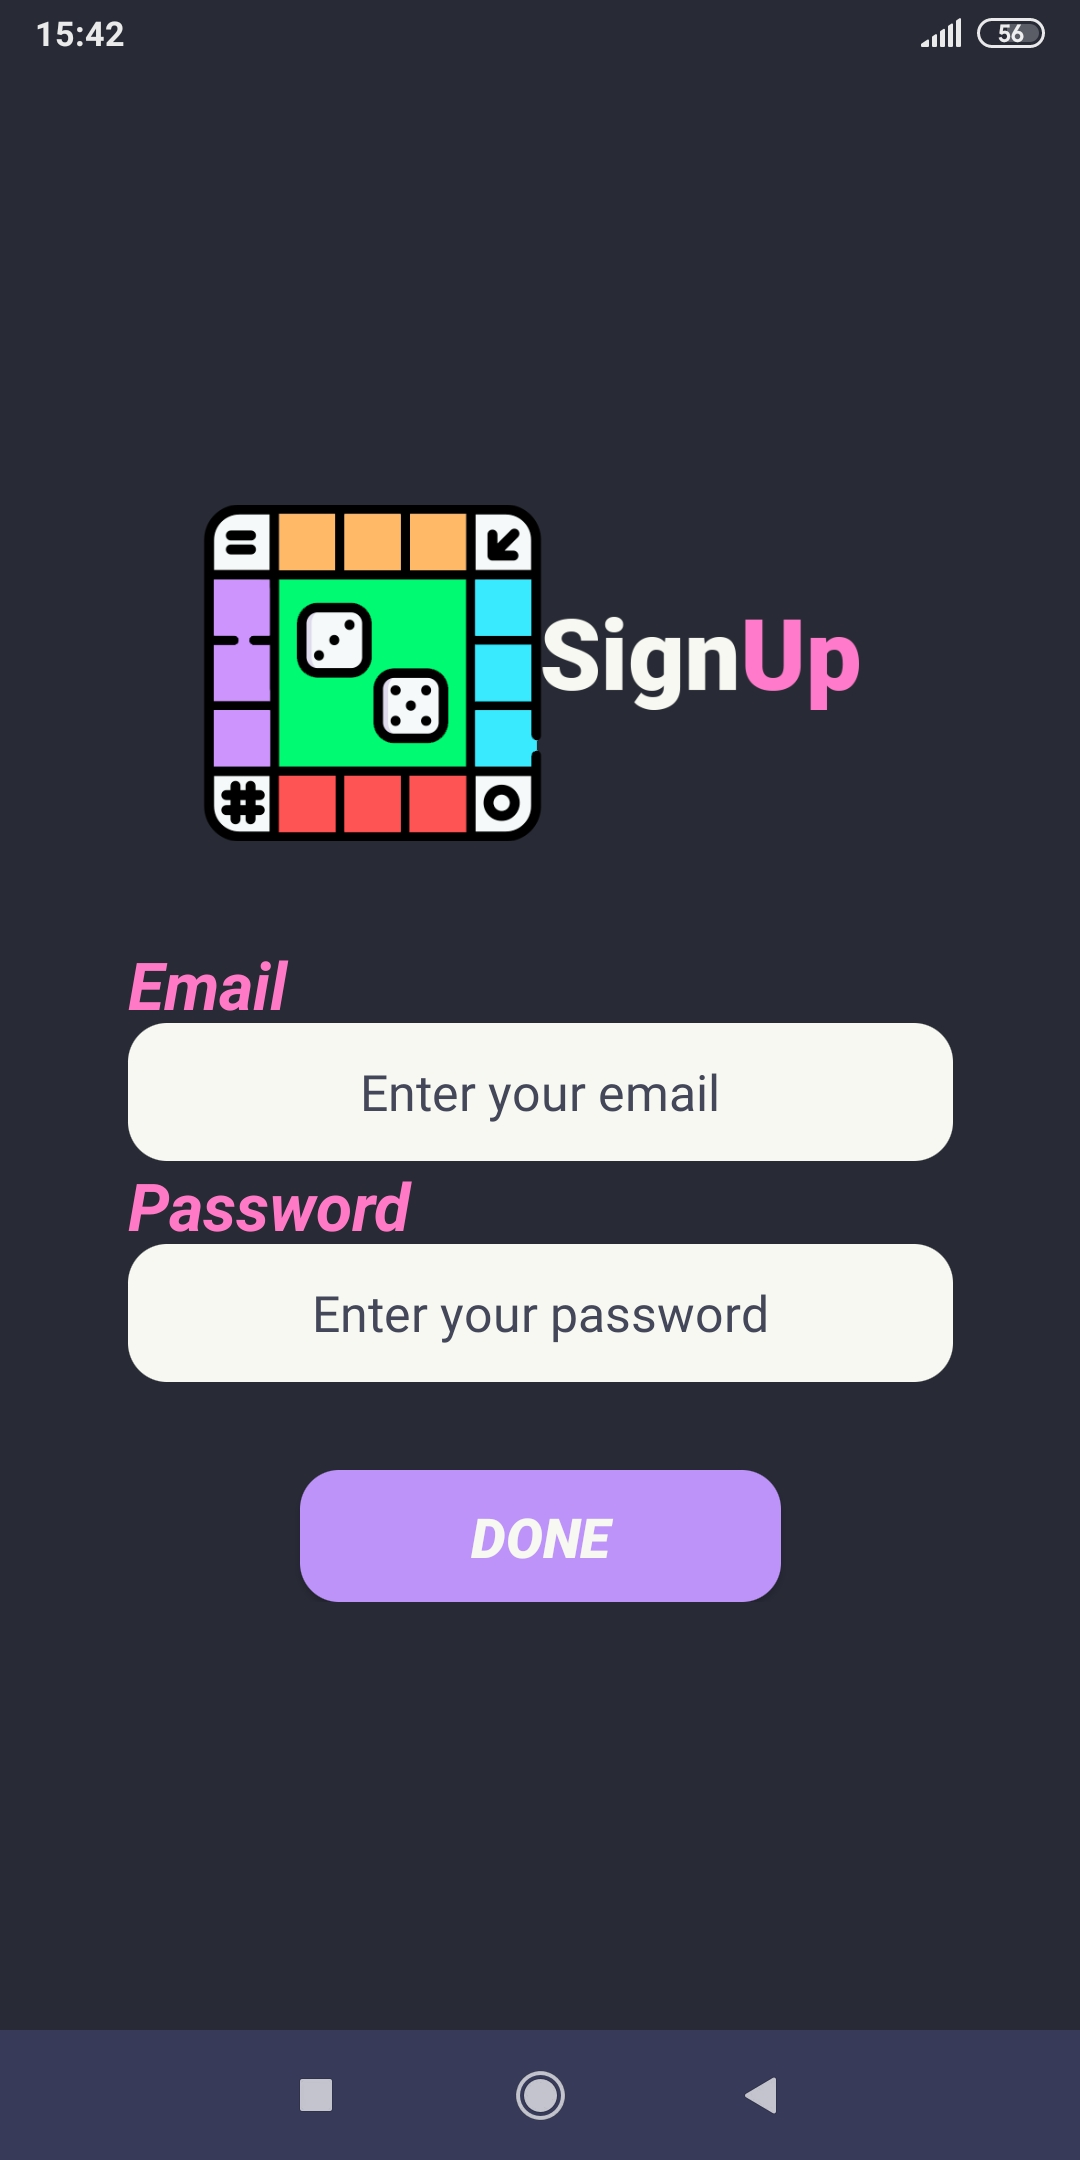
\includegraphics[width=0.5\linewidth]{fig/Capturas de pantalla de la aplicación/registro de cuenta.jpg}
    \caption{Registro de usuario}
    \label{fig:registro usuario}
\end{figure}

\section{Actividad principal}

Una vez iniciada la sesión, lo primero que ve el usuario es una lista vacía que rellenará él mismo con los juegos que vaya seleccionando. Estos juegos serán seleccionados uno a uno desde otra actividad que se hablará más adelante. Esta será accesible mediante un botón en la parte superior de la actividad.

Cuando tengamos juegos visibles en esta lista, esos juegos podrán ser clicados, lo cual hará que se nos abra otra actividad para ver el número de partidas, victorias y derrotas que llevemos en ese juego, aparte de otros tres botones que también se explicarán más adelante.

Además, nos encontraremos con una barra de navegación en la parte inferior de la pantalla con la que podremos movernos entre las distintas actividades y también cerrar sesión.


\begin{figure}[H]
    \centering
    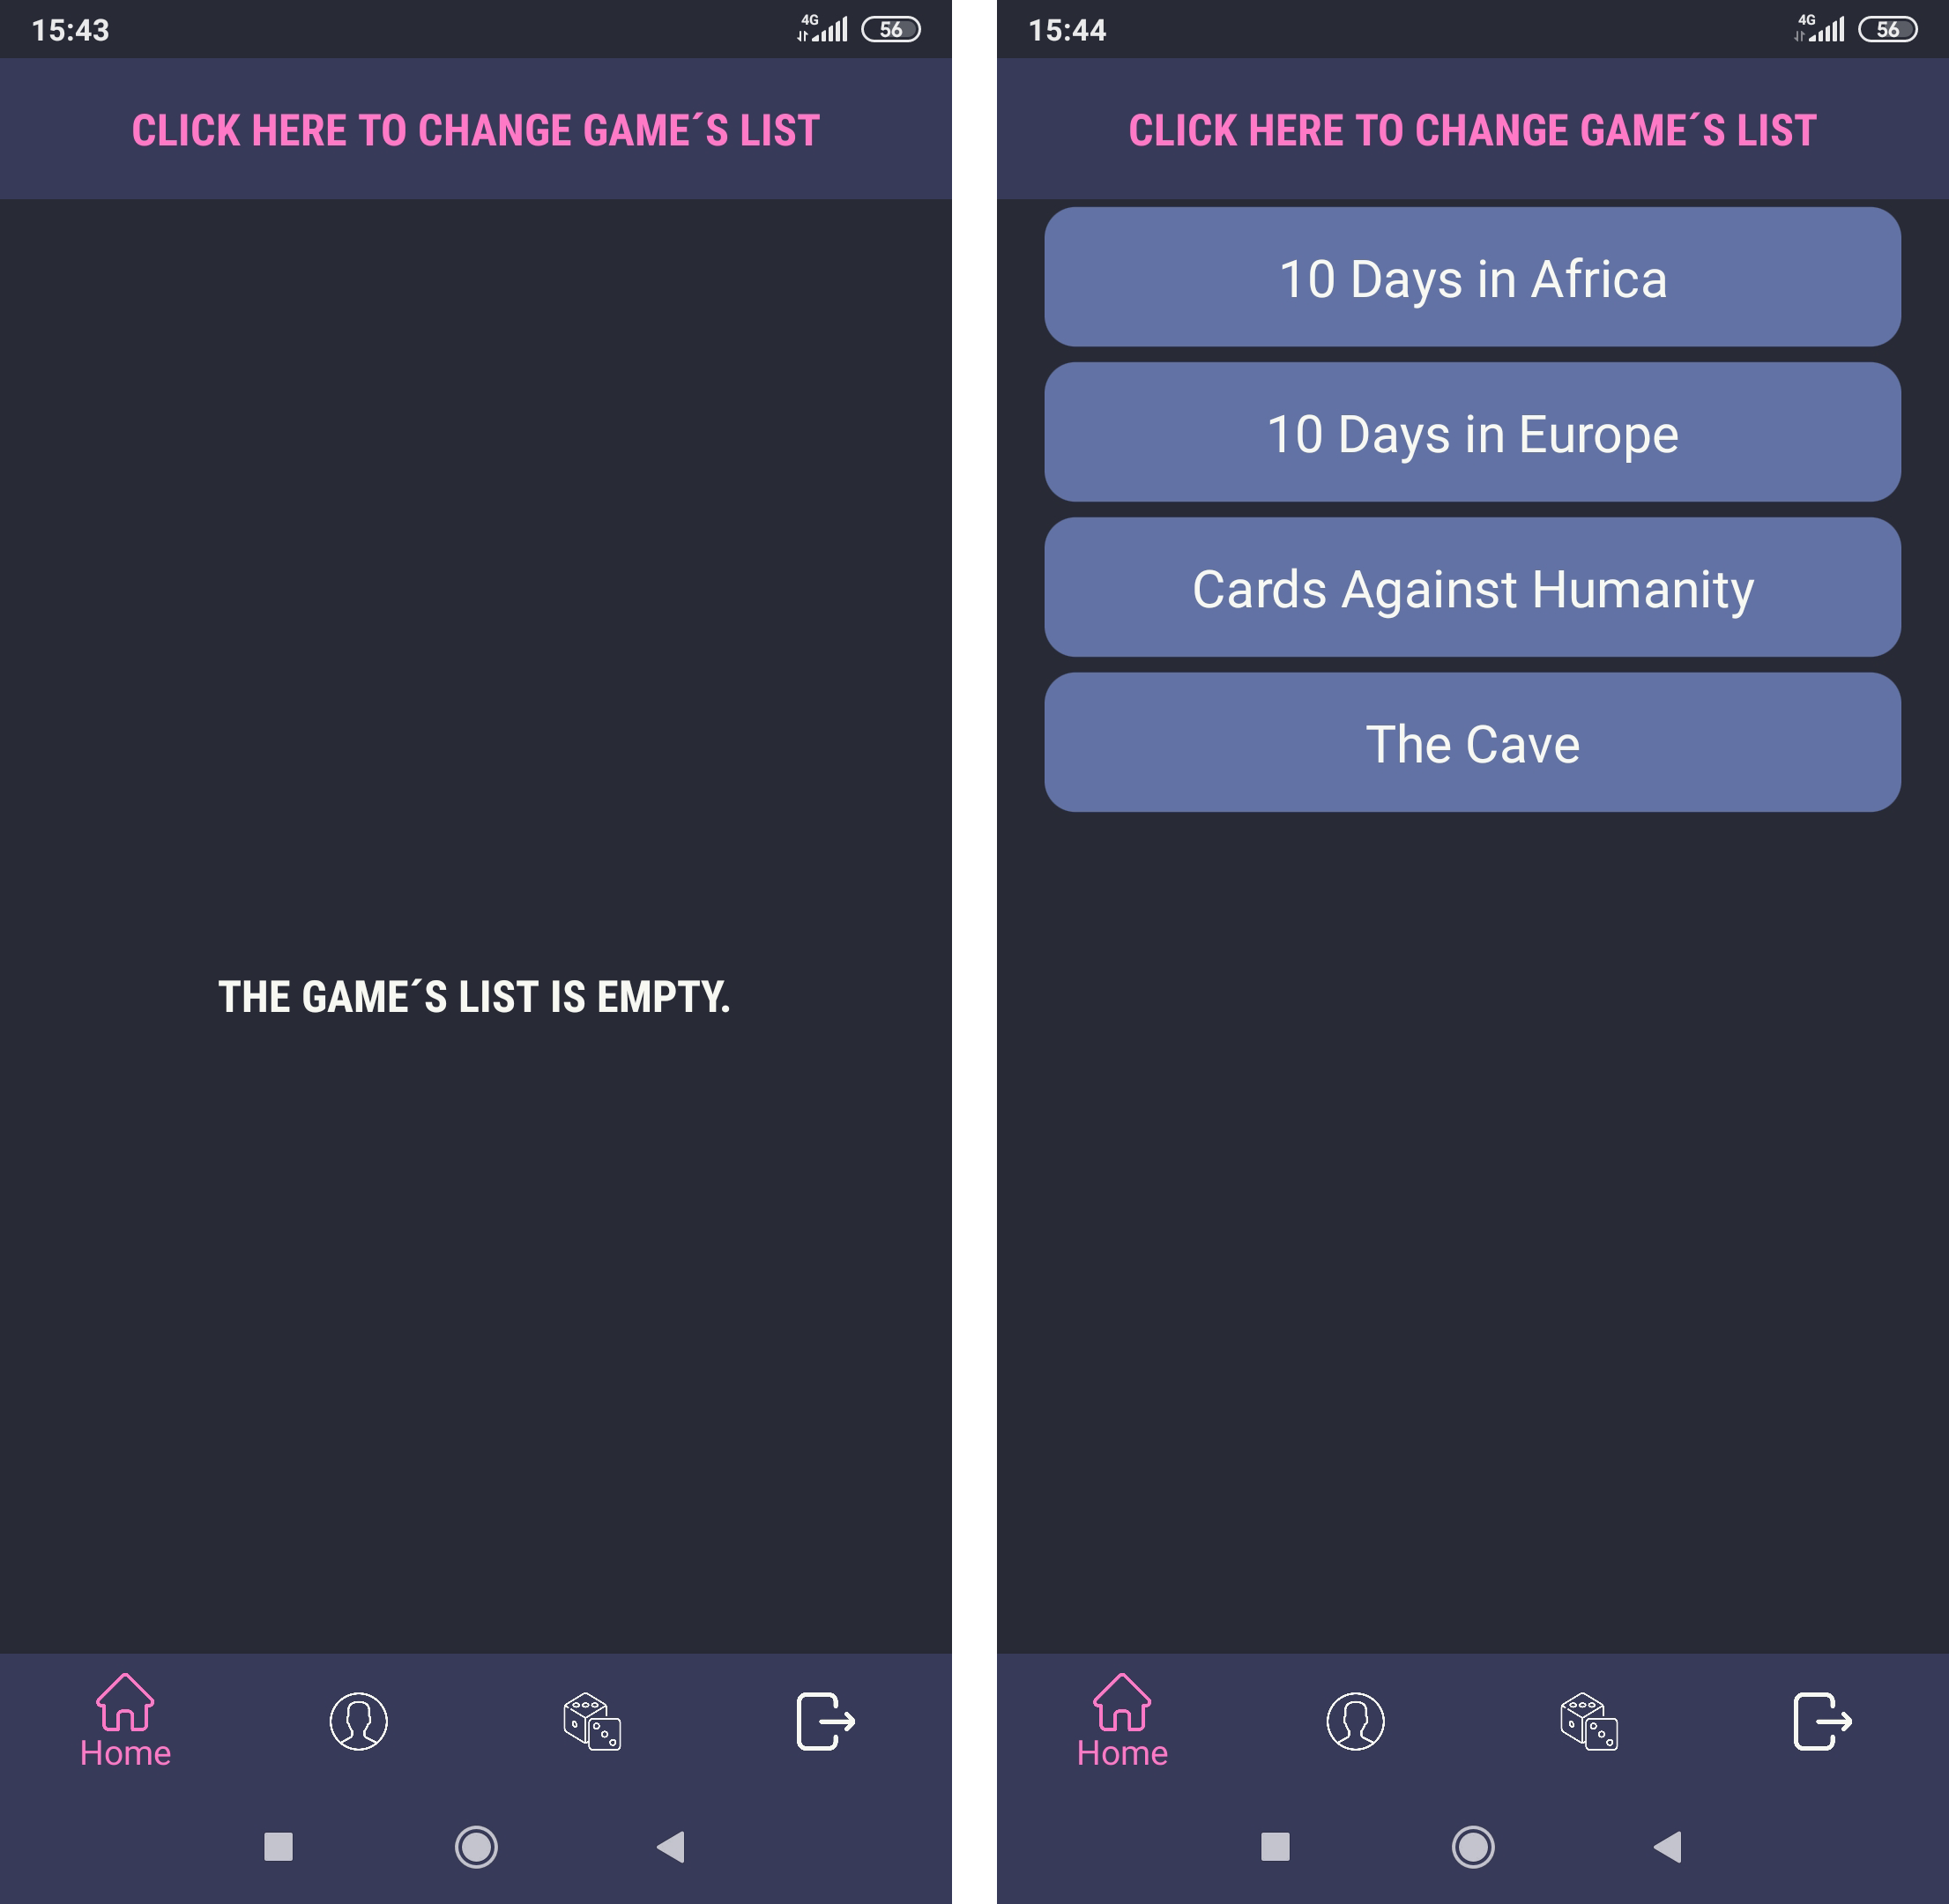
\includegraphics[width=1\linewidth]{fig/Capturas de pantalla de la aplicación/actividad principal.png}
    \caption{Actividad principal}
    \label{fig:actividad principal}
\end{figure}

\subsection{Registro de juegos favoritos}\label{cap:Actividad principal}

Una vez iniciada la sesión, lo primero que ve el usuario es una lista vacía que rellenará él mismo con los juegos que vaya seleccionando. Estos juegos serán seleccionados uno a uno desde otra actividad que se hablará más adelante. Esta será accesible mediante un botón en la parte superior de la actividad.

Cuando tengamos juegos visibles en esta lista, esos juegos podrán ser clicados, lo cual hará que se nos abra otra actividad para ver el número de partidas, victorias y derrotas que llevemos en ese juego, aparte de otros tres botones que también se explicarán más adelante.

Además, nos encontraremos con una barra de navegación en la parte inferior de la pantalla con la que podremos movernos entre las distintas actividades y también cerrar sesión.


\begin{figure}[H]
    \centering
    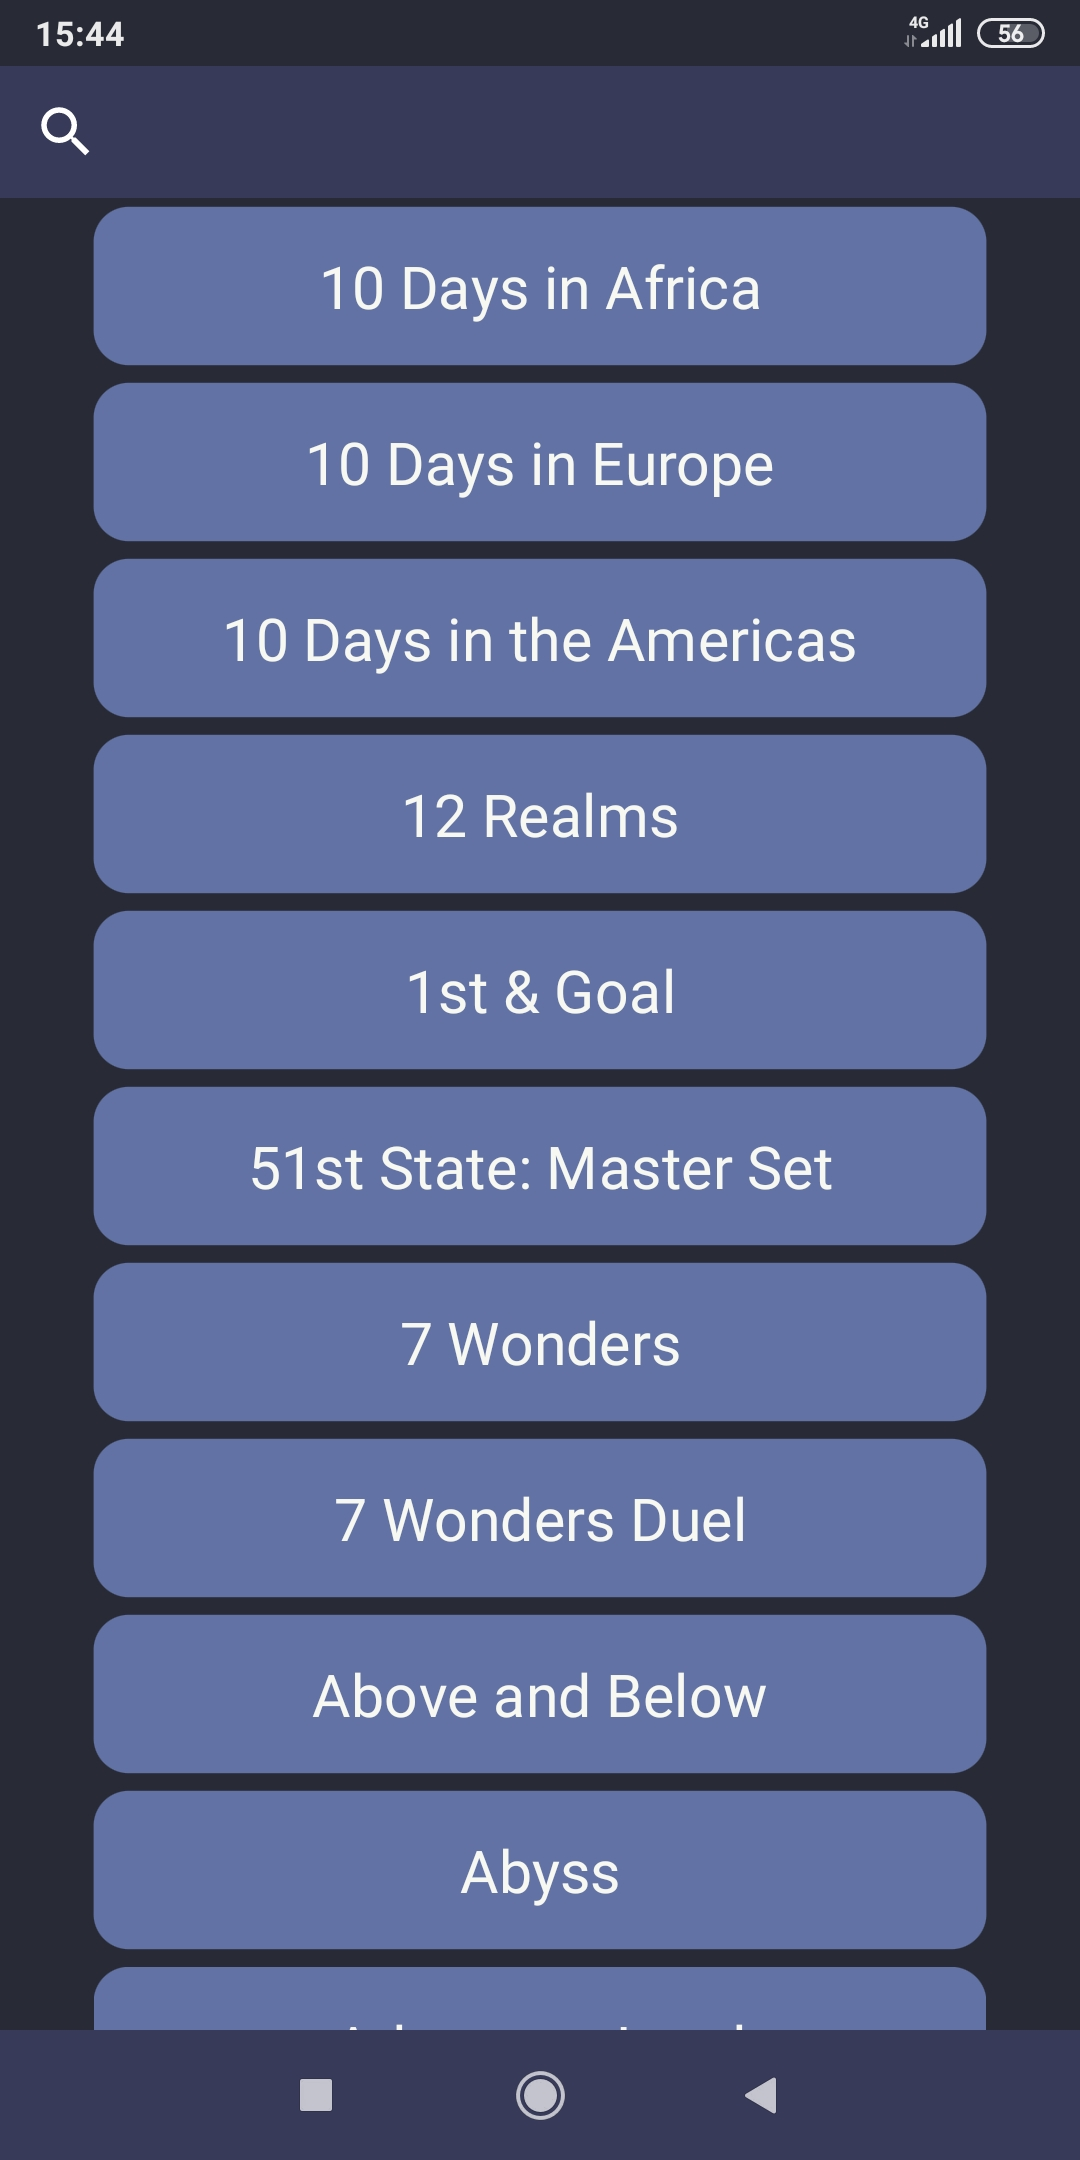
\includegraphics[width=0.5\linewidth]{fig/Capturas de pantalla de la aplicación/anadir juegos favoritos.jpg}
    \caption{Registro de juegos favoritos}
    \label{fig:registro juegos favoritos}
\end{figure}

\subsection{Actividades clicando juegos}

Una vez clicado algún juego, ya sea favorito o no, se nos abrirá una actividad con las estadísticas de partidas, victorias y derrotas en ese juego, y algunos botones con diferentes funcionalidades.

El único cambio que veremos en si es favorito o no el juego será en las funcionalidades de esos botones. Si el juego es clicado desde la lista de todos los juegos sacados de la API, solamente veremos un único botón que hará que añadamos ese juego a tu lista de juegos favoritos. En cambio, si es clicado desde nuestra lista de juegos favoritos, veremos tres botones con los que podremos eliminar el juego de esa lista, añadir una partida nueva y ver las partidas anteriormente jugadas.

\begin{figure}[H]
    \centering
    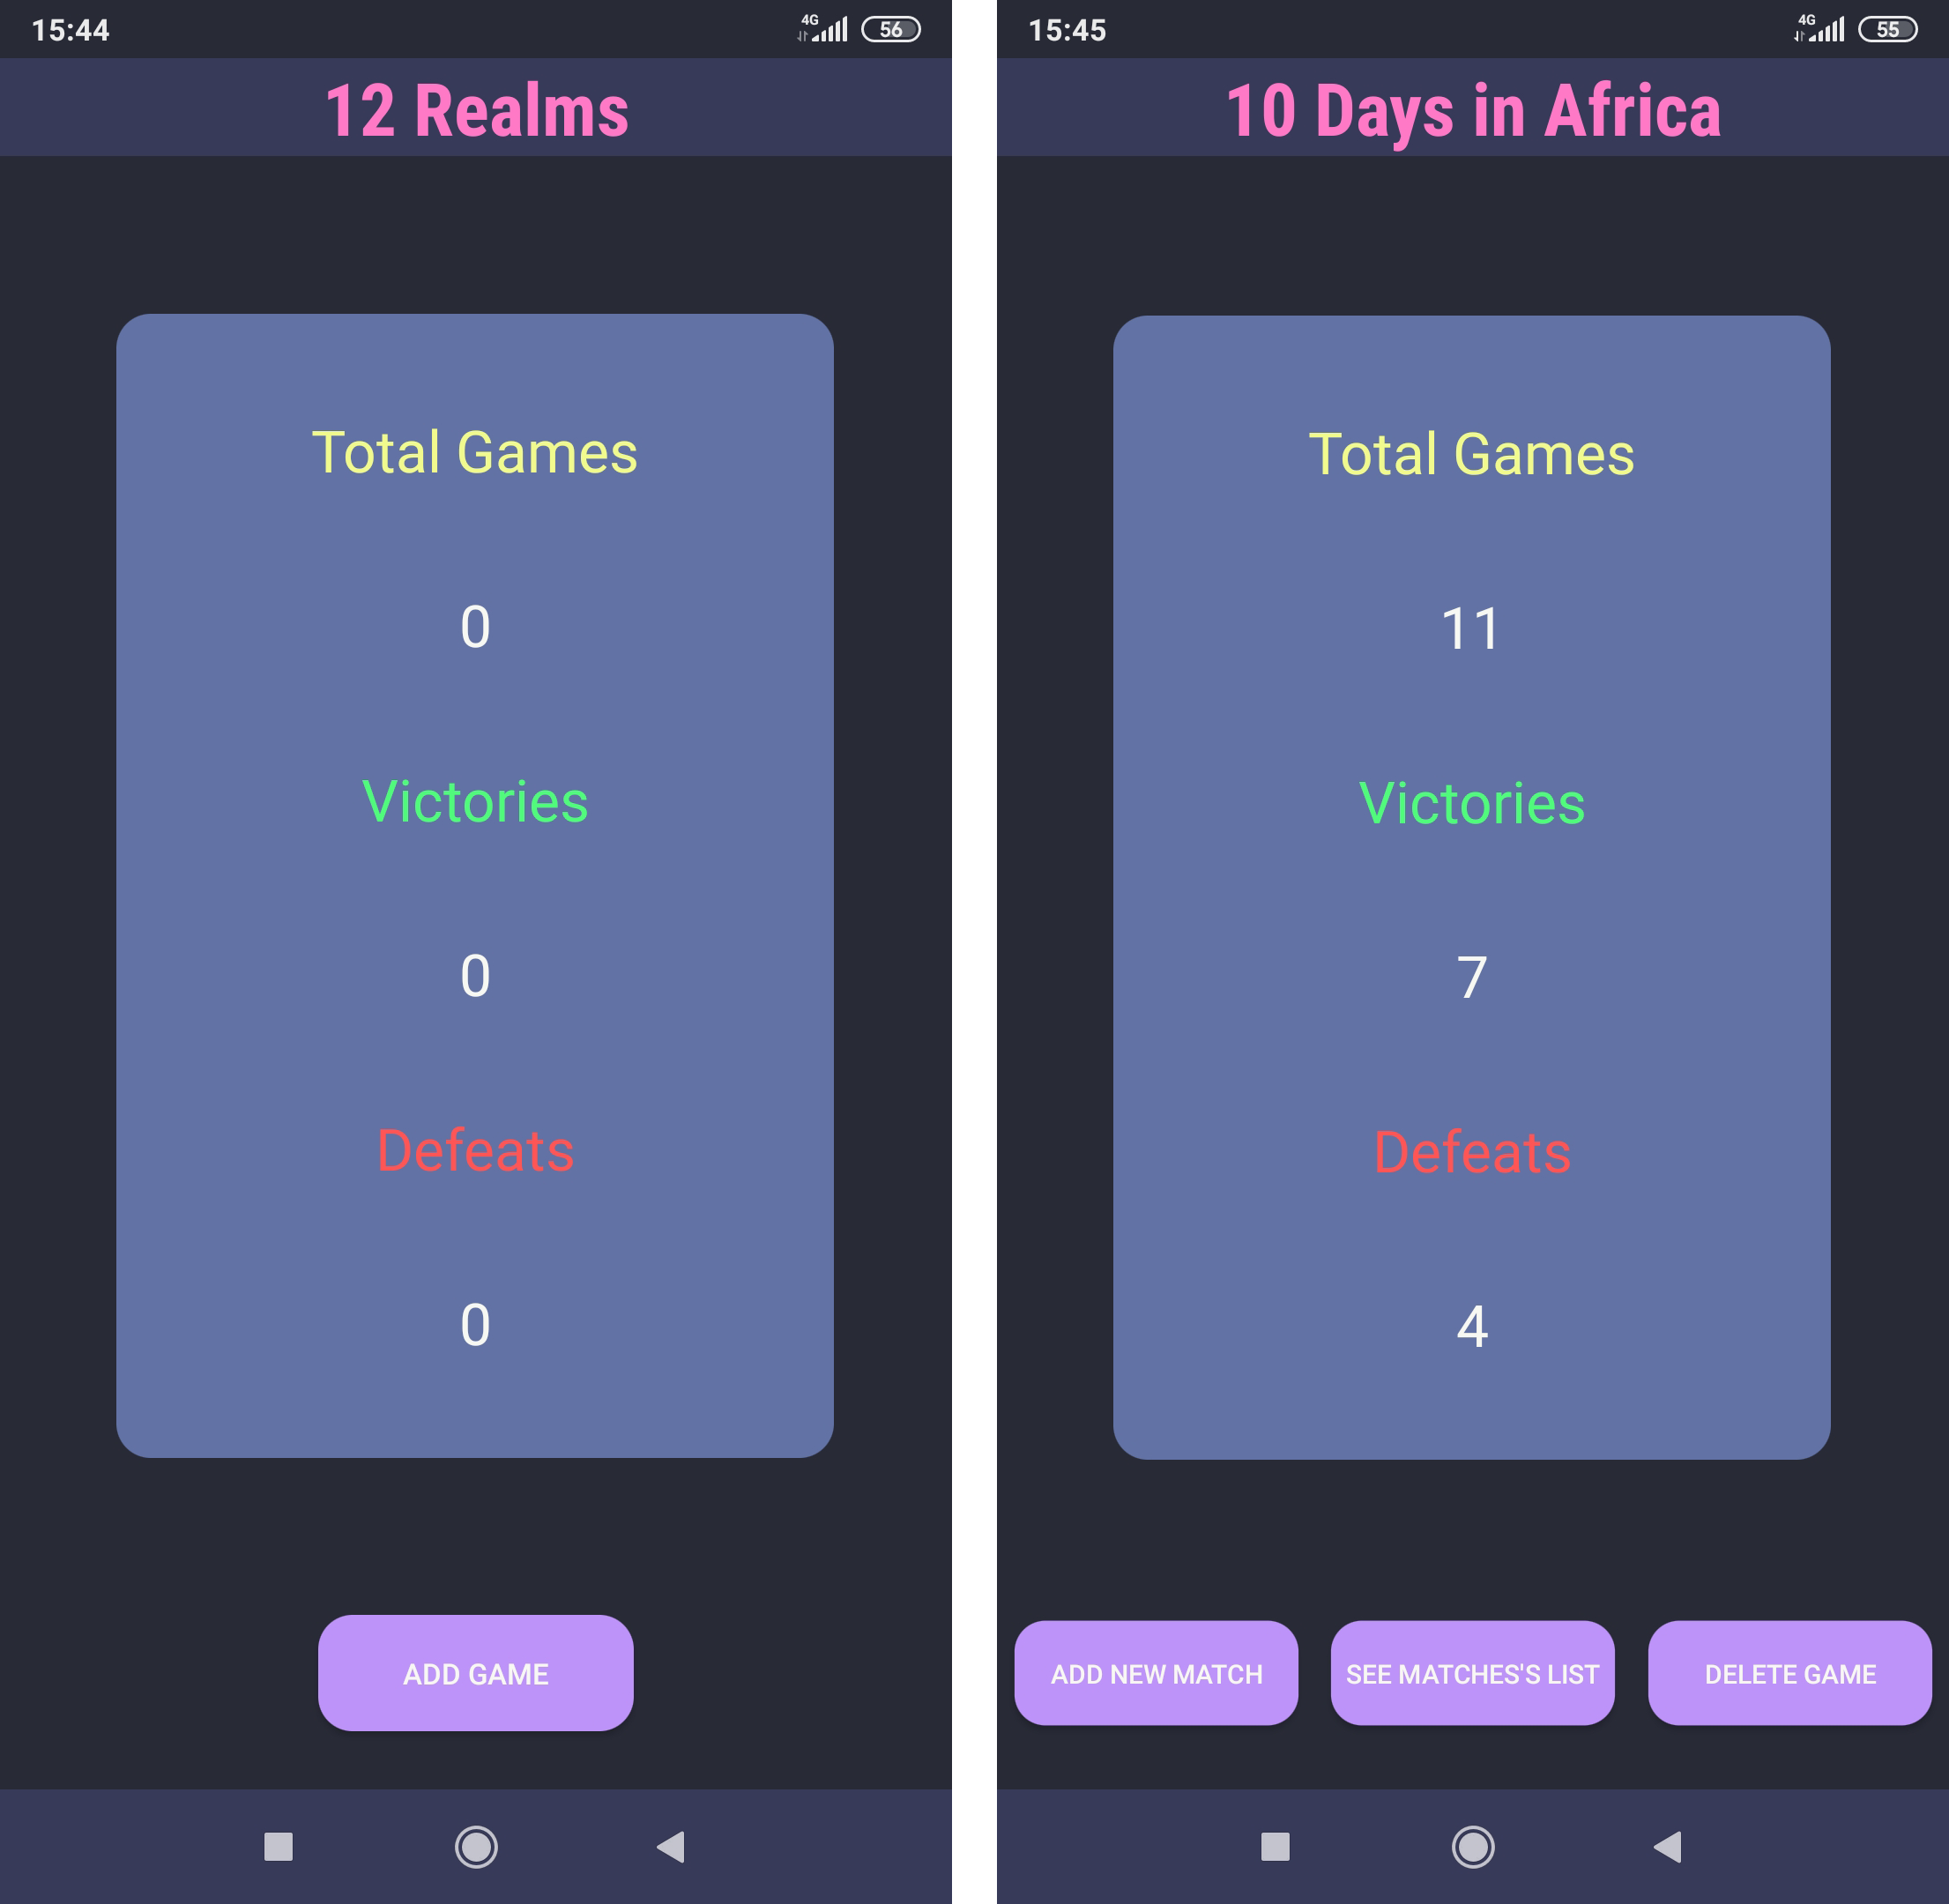
\includegraphics[width=1\linewidth]{fig/Capturas de pantalla de la aplicación/juegos clicados.png}
    \caption{Actividades clicando juegos}
    \label{fig:actividades clicando juegos}
\end{figure}

\subsection{Registro de nuevas partidas}

Si le damos al botón para añadir nuevas partidas mencionado anteriormente, se nos abrirá una nueva actividad donde podremos añadir hasta ocho jugadores, los cuales serán autor rellenados haciendo uso de la base de datos, con sus puntuaciones. El primer jugador siempre será el usuario que cree la partida.

\begin{figure}[H]
    \centering
    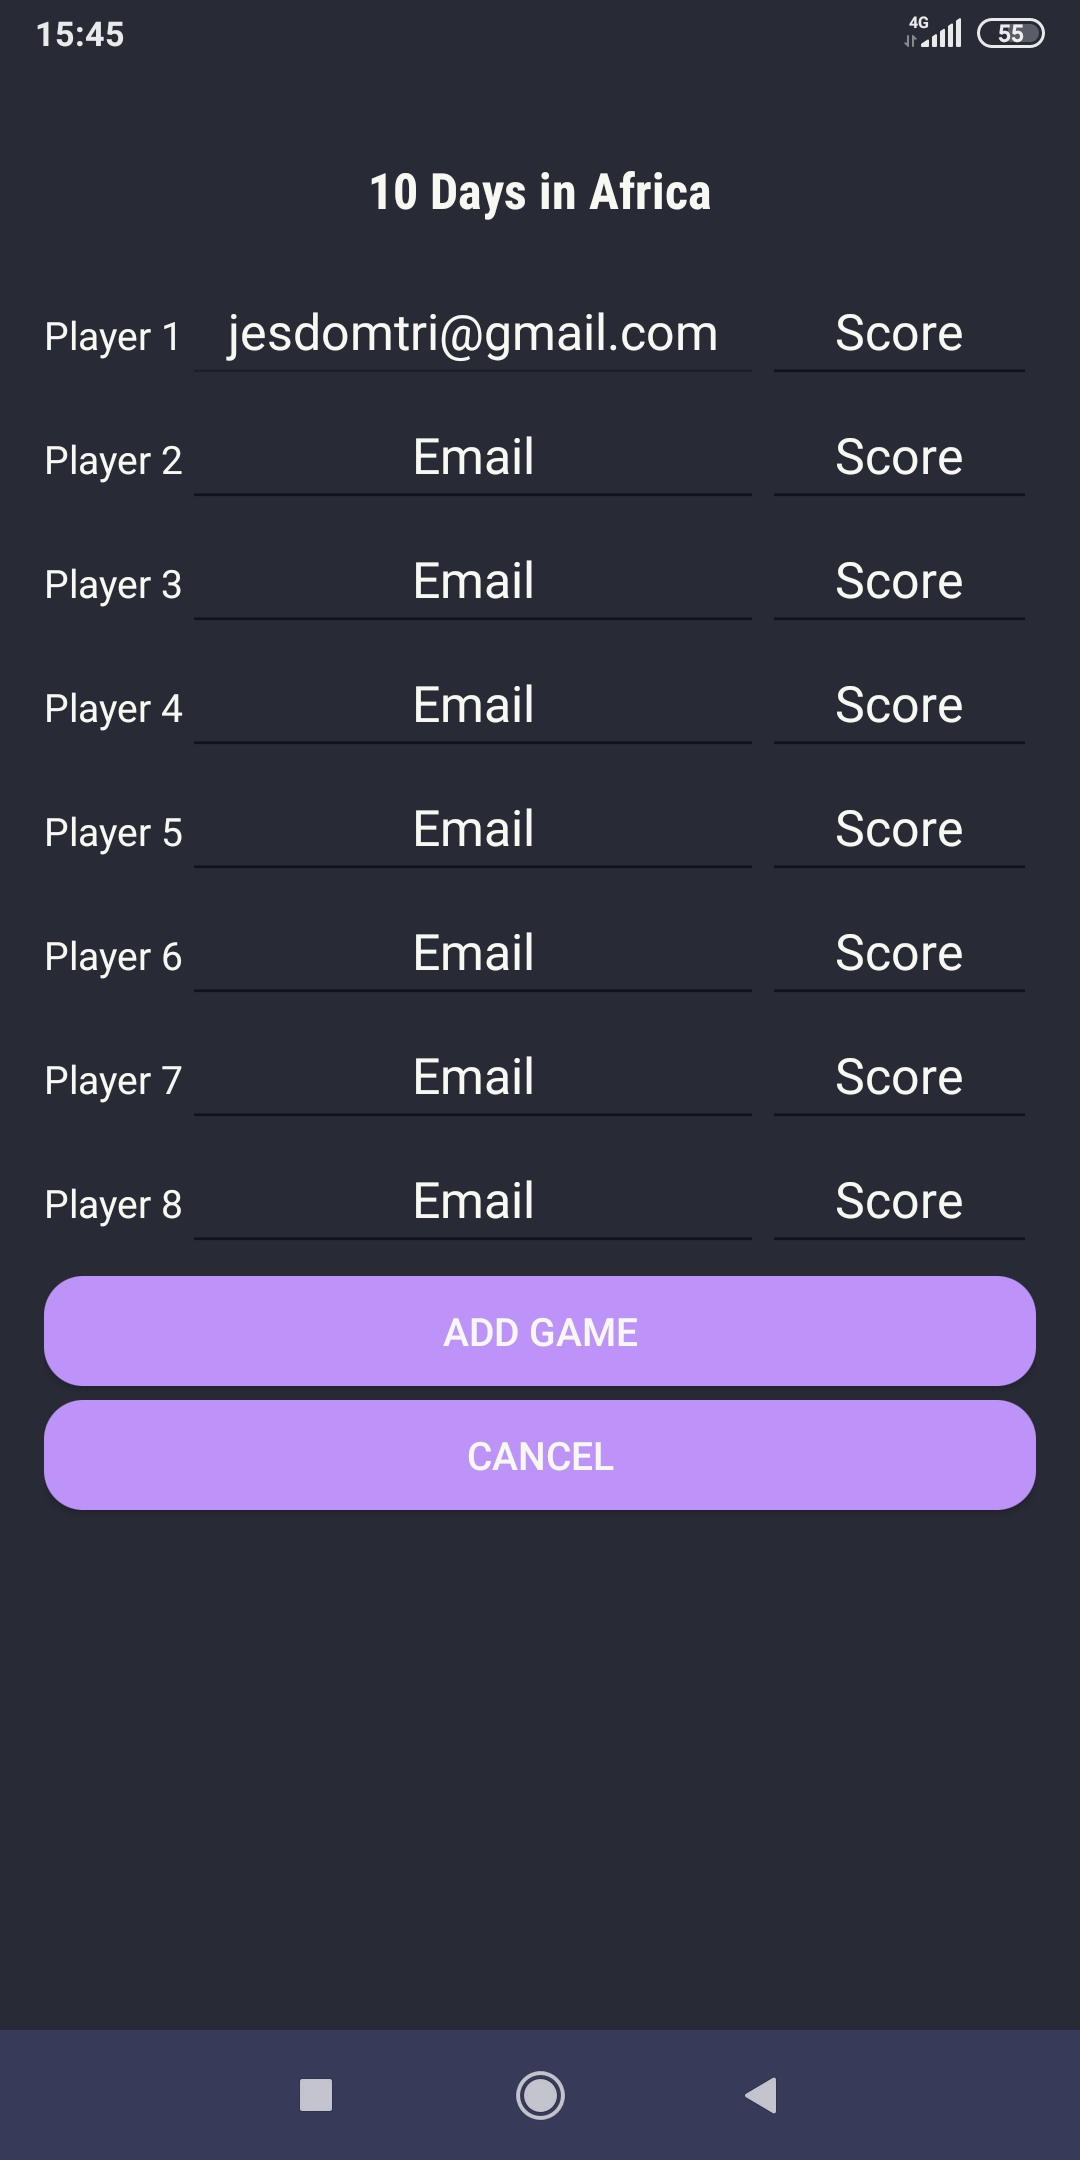
\includegraphics[width=0.5\linewidth]{fig/Capturas de pantalla de la aplicación/anadir partidas.jpg}
    \caption{Registro de nuevas partidas}
    \label{fig:registro de nuevas partidas}
\end{figure}

\subsection{Listado de partidas}

En cambio, si le damos al botón para ver el listado de partidas que llevamos en ese juego, veremos una lista con una interfaz minimalista donde encontraremos cada partida de forma independiente donde se nos marcará nuestra puntuación, posición y una corona de color amarillo si nuestra posición es el primer lugar.

\begin{figure}[H]
    \centering
    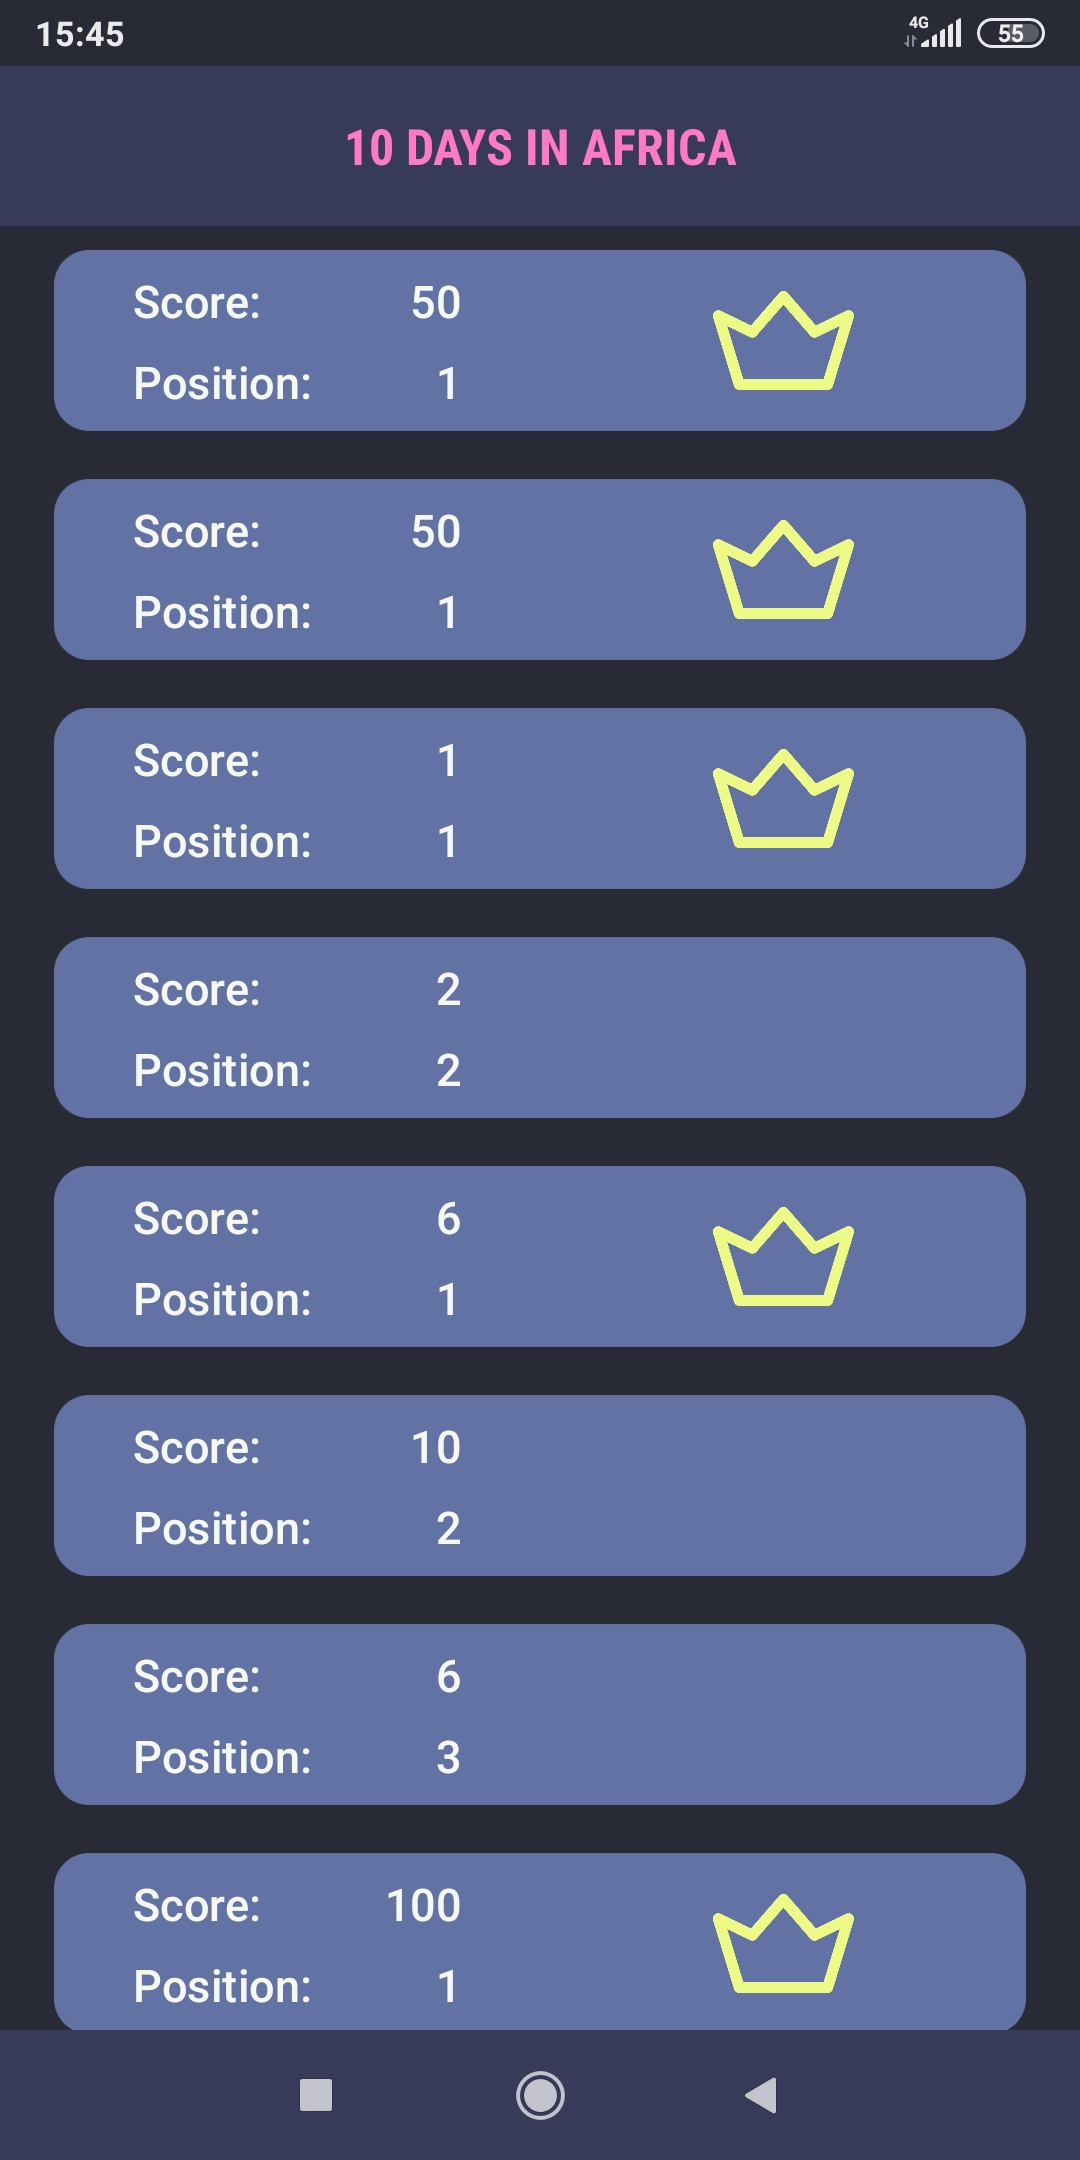
\includegraphics[width=0.5\linewidth]{fig/Capturas de pantalla de la aplicación/lista de partidas.jpg}
    \caption{Listado de partidas}
    \label{fig:listado de partidas}
\end{figure}

\section{Actividad de datos de usuario}

La segunda actividad que podrá ser clicada en la barra de navegación será una actividad donde el usuario se encontrará con los datos de su perfil como puede ser el correo electrónico, la contraseña en forma de asteriscos, un botón para cambiar su contraseña mediante un correo que se le enviará al correo electrónico, el identificador del usuario y la fecha de creación de la cuenta.

\begin{figure}[H]
    \centering
    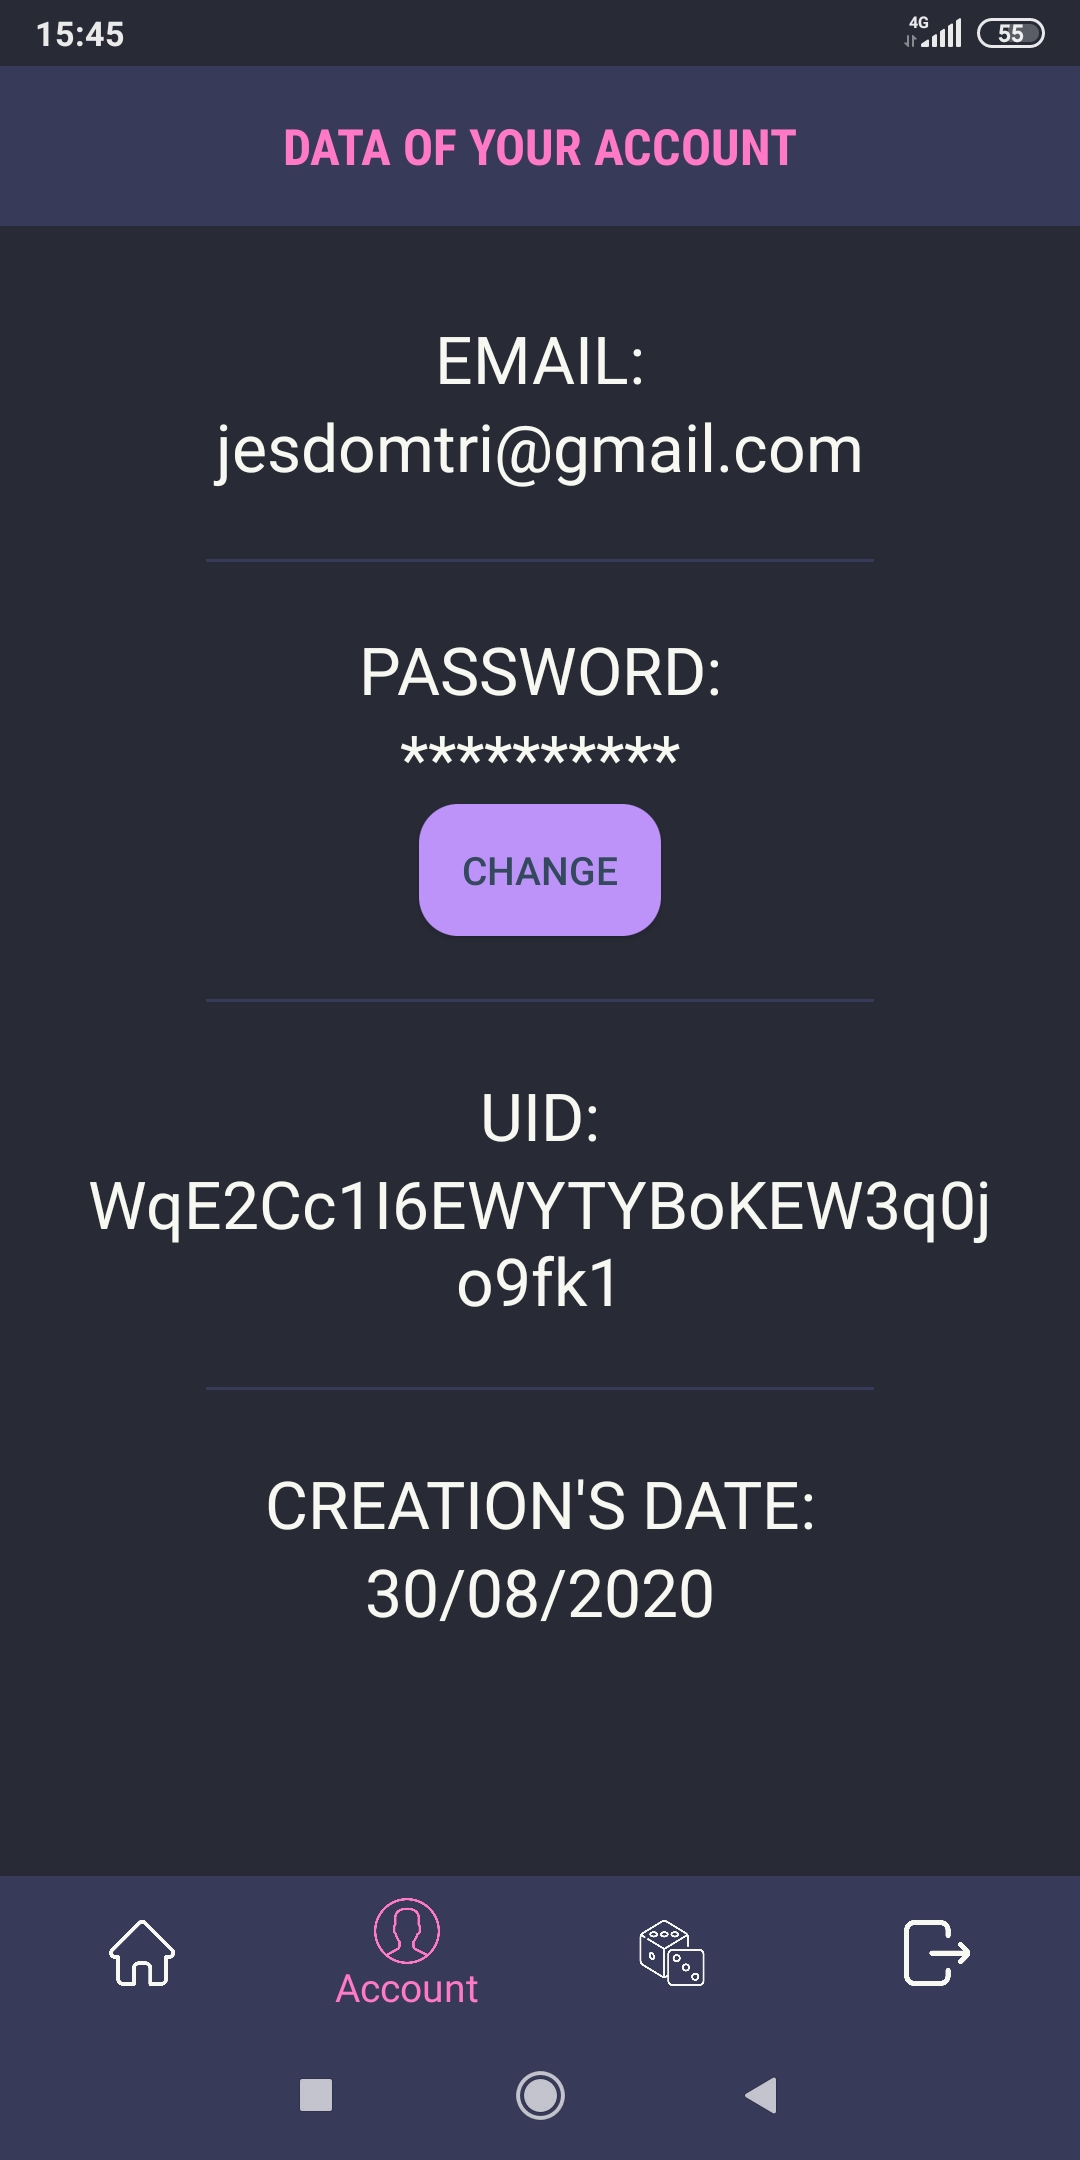
\includegraphics[width=0.5\linewidth]{fig/Capturas de pantalla de la aplicación/actividad datos usuario.jpg}
    \caption{Actividad de datos de usuario}
    \label{fig:actividad datos usuario}
\end{figure}

\section{Actividad de utilidades}

La última actividad localizada en la barra de navegación es la actividad donde se encuentran las distintas utilidades que se podrán usar en el transcurso de la partida. En esta actividad encontraremos 4 utilidades las cuales serán descritas una a una a continuación.

\begin{figure}[H]
    \centering
    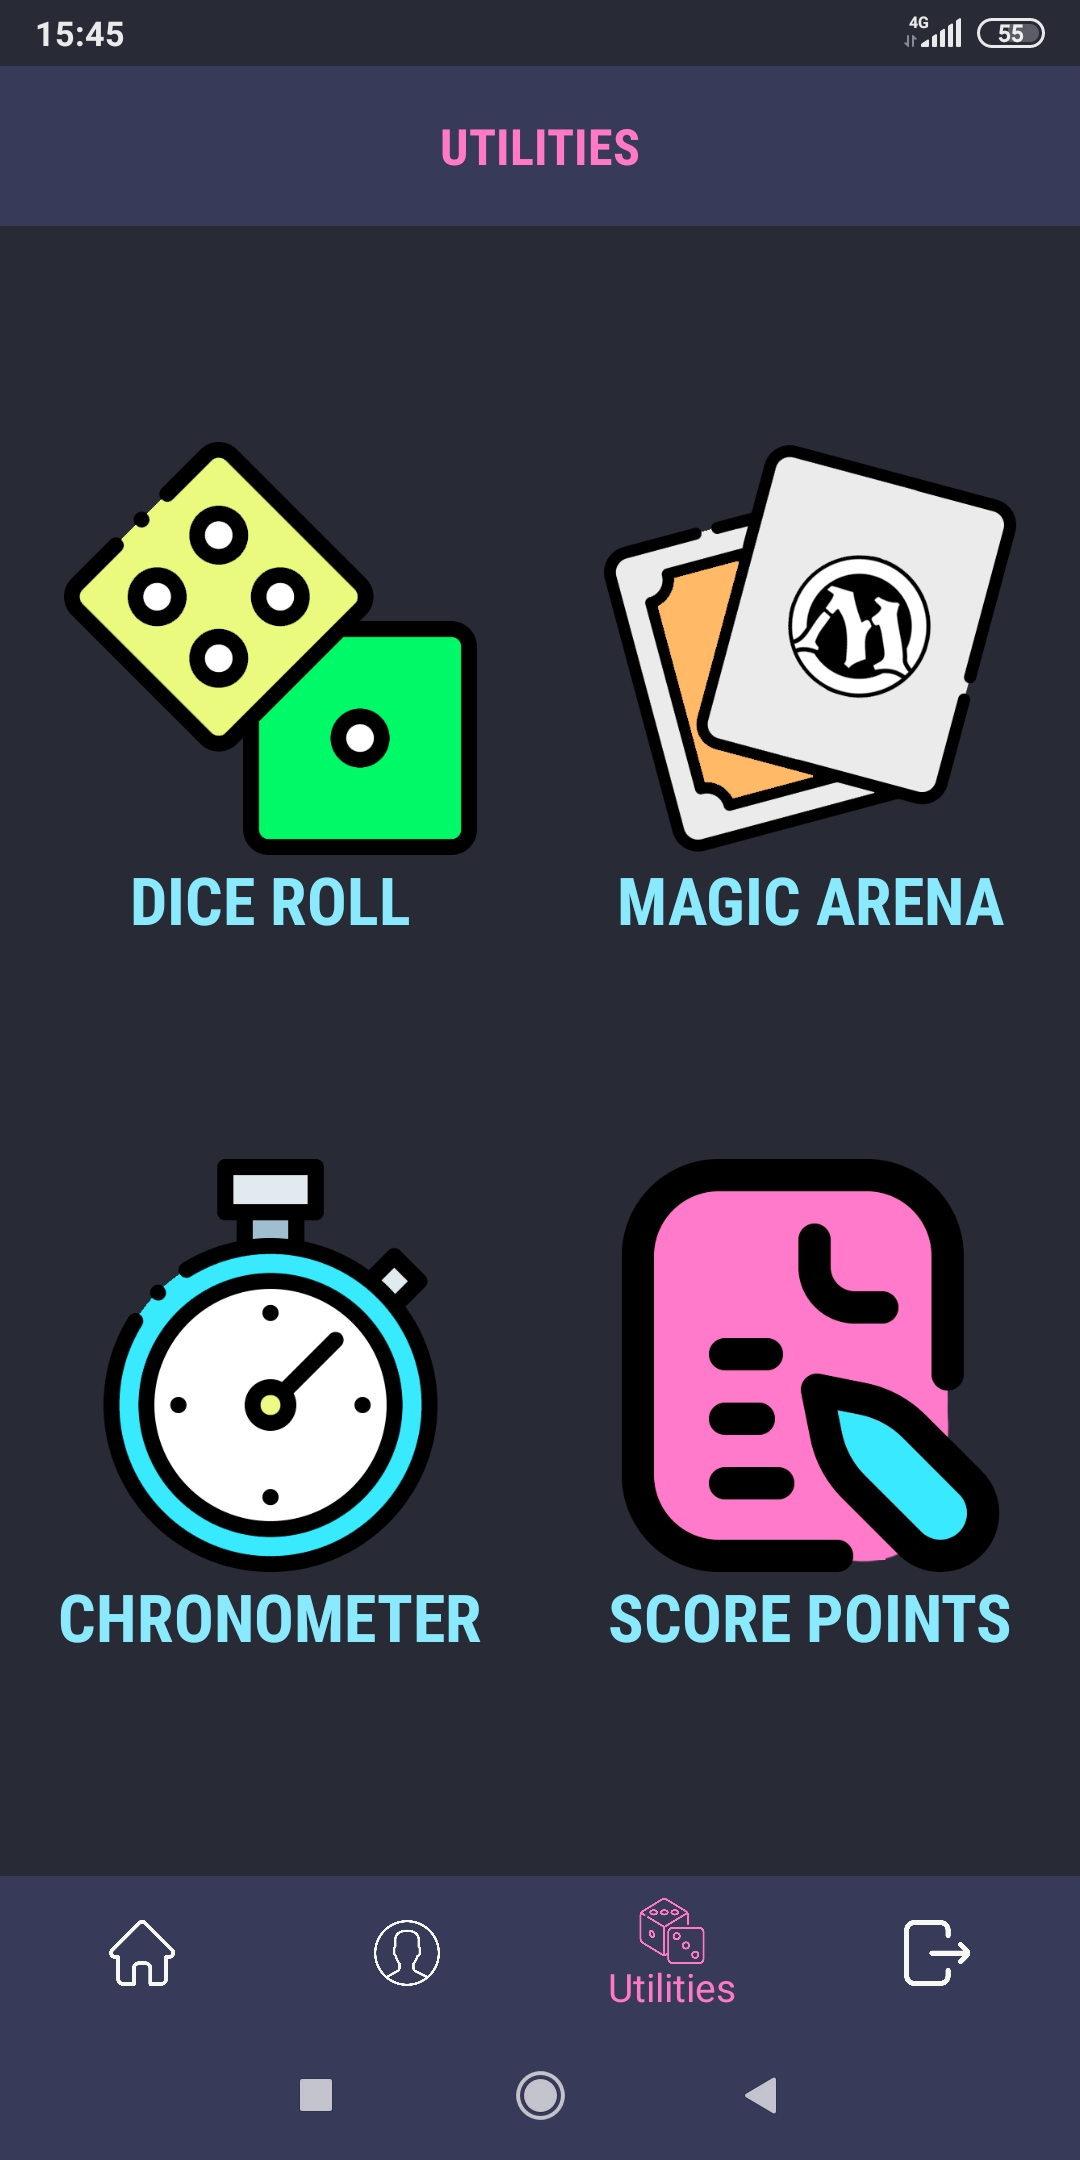
\includegraphics[width=0.5\linewidth]{fig/Capturas de pantalla de la aplicación/actividad utilidades.jpg}
    \caption{Actividad de utilidades}
    \label{fig:actividad utilidades}
\end{figure}

\subsection{Lanzamiento de dados}\label{cap:Actividad de utilidades}

En esta primera utilidad nos encontraremos con un número que van a ser los dados que queramos lanzar el cual va desde 1 a 20. Debajo de este número se encuentran los tres tipos de dados que vamos a utilizar representados por una imagen de cada: 6, 12 y 20 caras. 

En la zona inferior tendremos el botón para lanzar los dados con la configuración que hayamos elegido anteriormente, cuyo botón, una vez pulsado, nos mostrará una lista vertical con una cantidad de imágenes igual al número de dados que elegimos mostrando de forma aleatoria las distintas caras del dado predefinido. 

\begin{figure}[H]
    \centering
    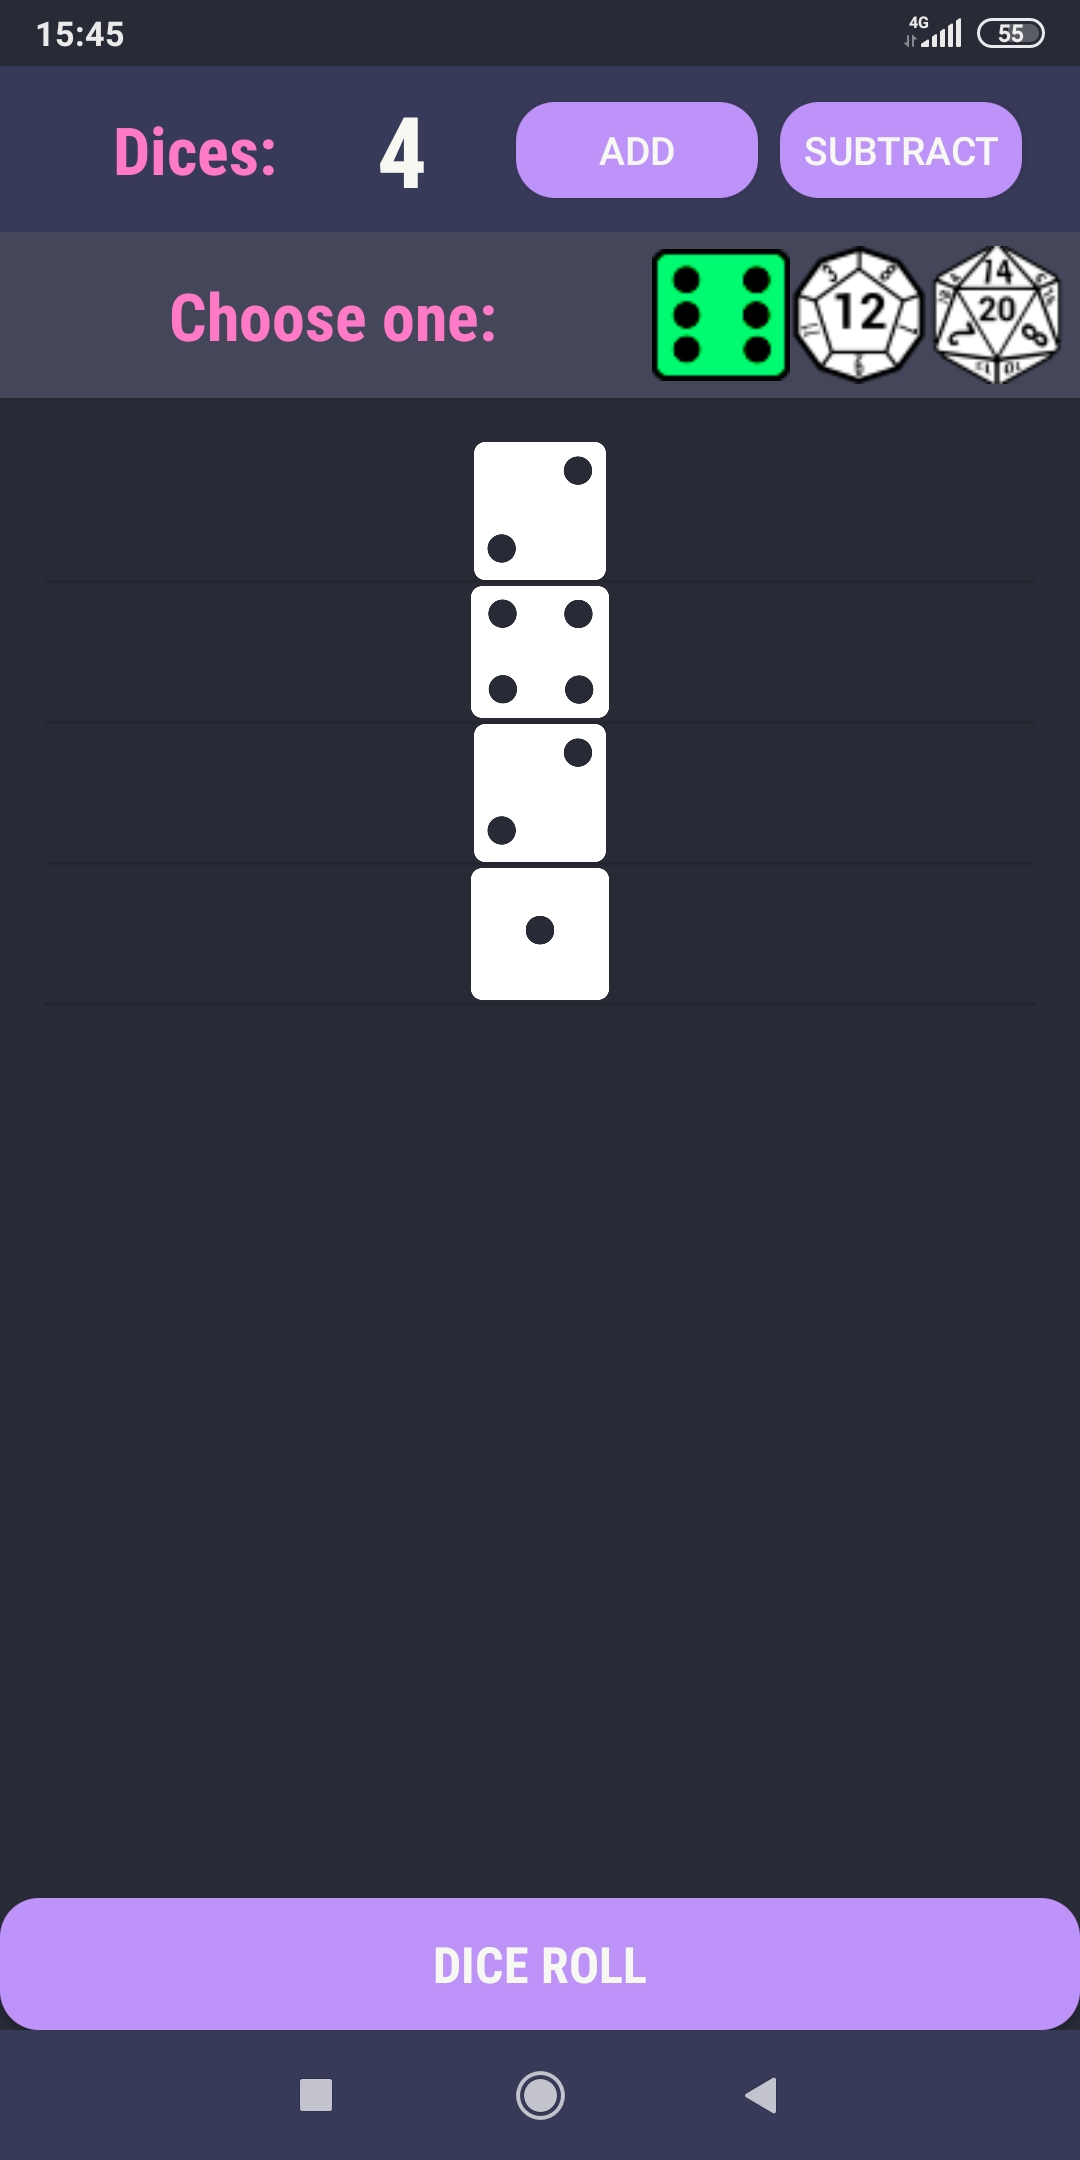
\includegraphics[width=0.5\linewidth]{fig/Capturas de pantalla de la aplicación/dice roll.jpg}
    \caption{Lanzamiento de dados}
    \label{fig:lanzamiento dados}
\end{figure}

\subsection{Magic Arena}

Para juegos de cartas como pueden ser las Magics se ha creado esta utilidad que cuenta con numerosos contadores para 4 jugadores como máximo en los que podremos ver reflejados los puntos de vida, maná, ataque, veneno, commander o lo que necesitemos dependiendo del juego, aparte de un botón para restablecer todos los contadores a 0 exceptuando los de vida que se ponen a 20. 

Estos contadores aumentan o disminuyen haciéndose uso de los botones que tenemos a los laterales. Los valores que se sumarán o restarán serán uno o cinco puntos.

\begin{figure}[H]
    \centering
    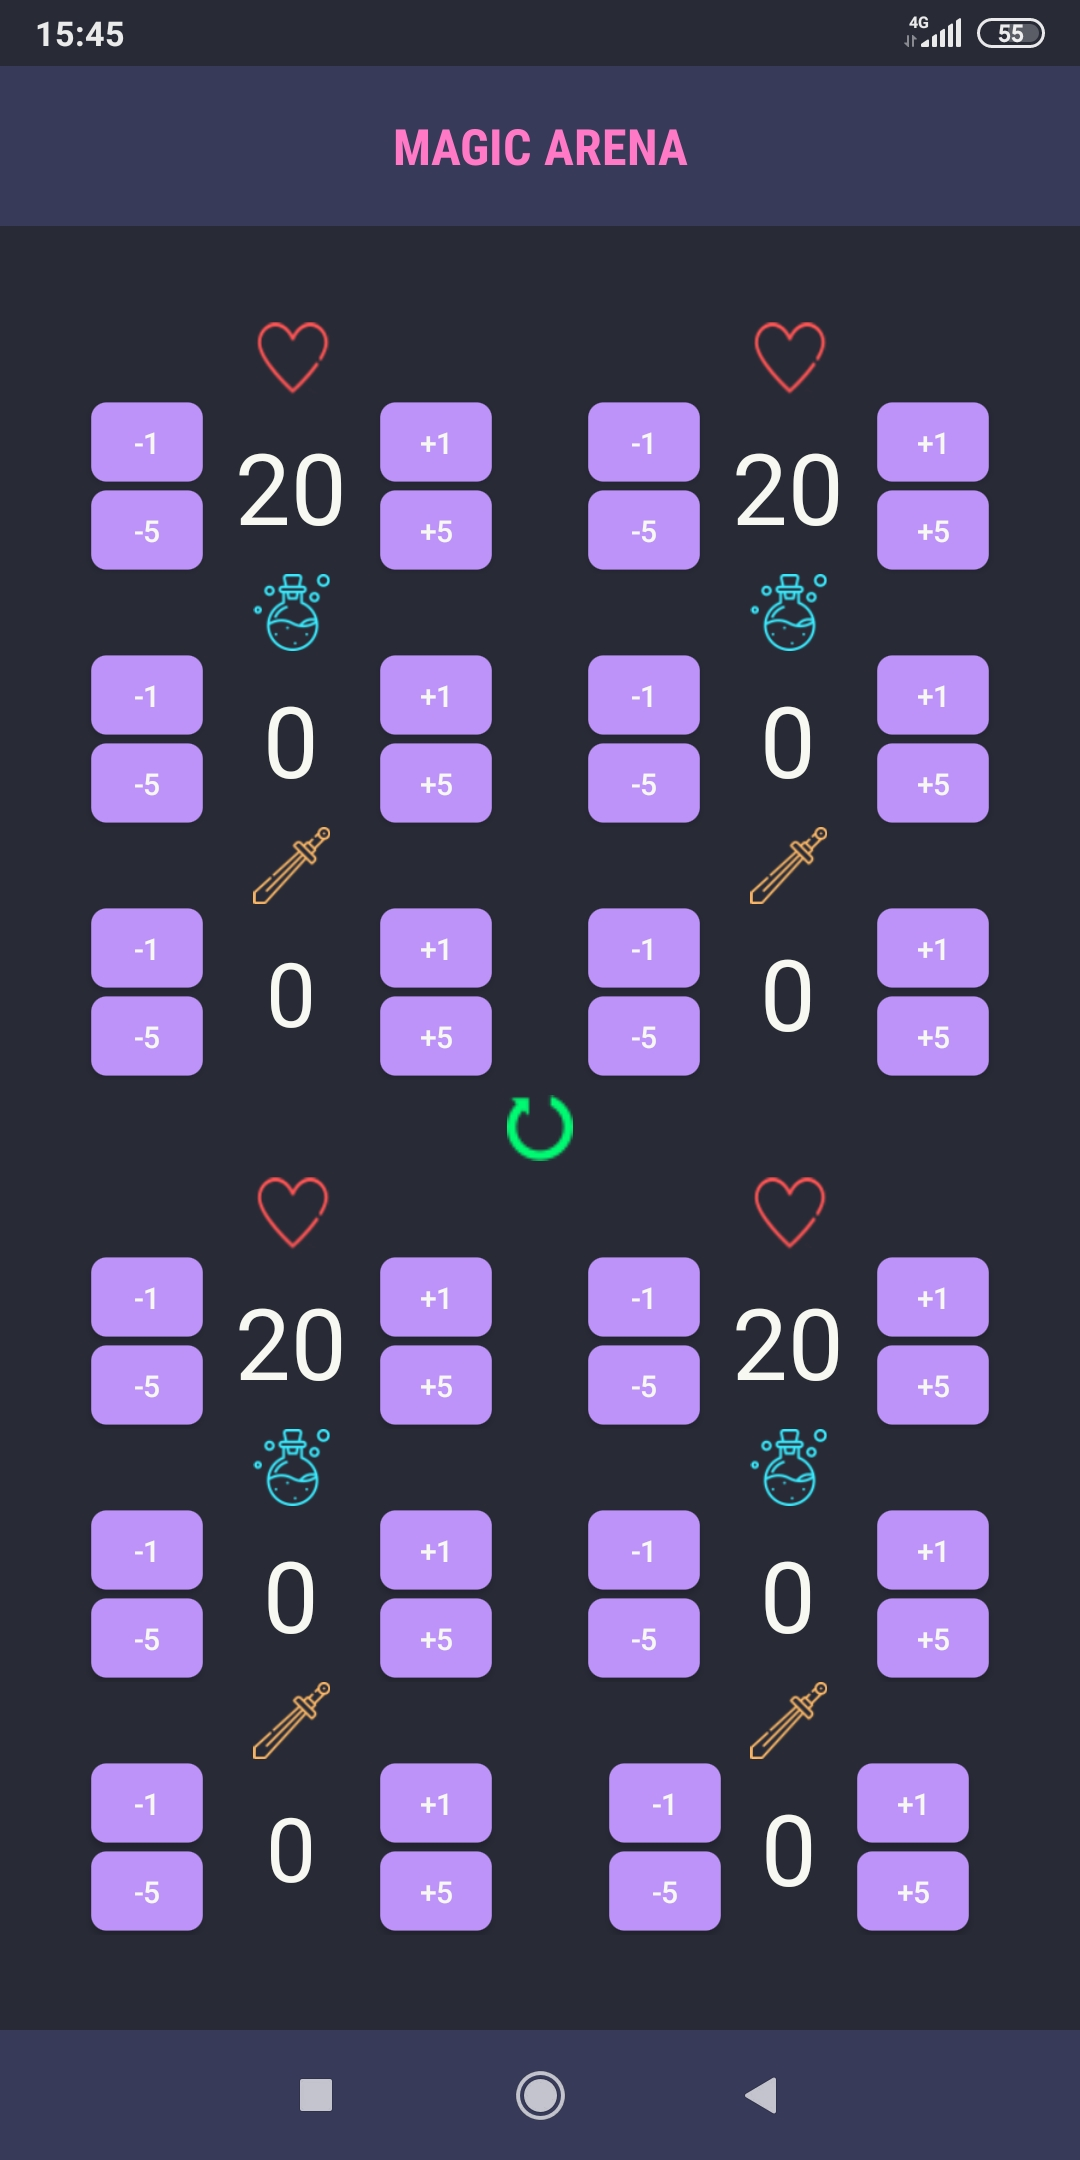
\includegraphics[width=0.5\linewidth]{fig/Capturas de pantalla de la aplicación/magic arena.jpg}
    \caption{Magic Arena}
    \label{fig:magic arena}
\end{figure}

\subsection{Cronometro}

Esta actividad, aunque es realmente básica y sencilla, se implementó con la idea de no depender de más aplicaciones o, simplemente, para no tener que salir de esta aplicación para cronometrar un tiempo.

Contamos con tres botones: inicio, pausa y reinicio; y un timer en el centro de la actividad que será lo que represente el tiempo transcurrido.


\begin{figure}[H]
    \centering
    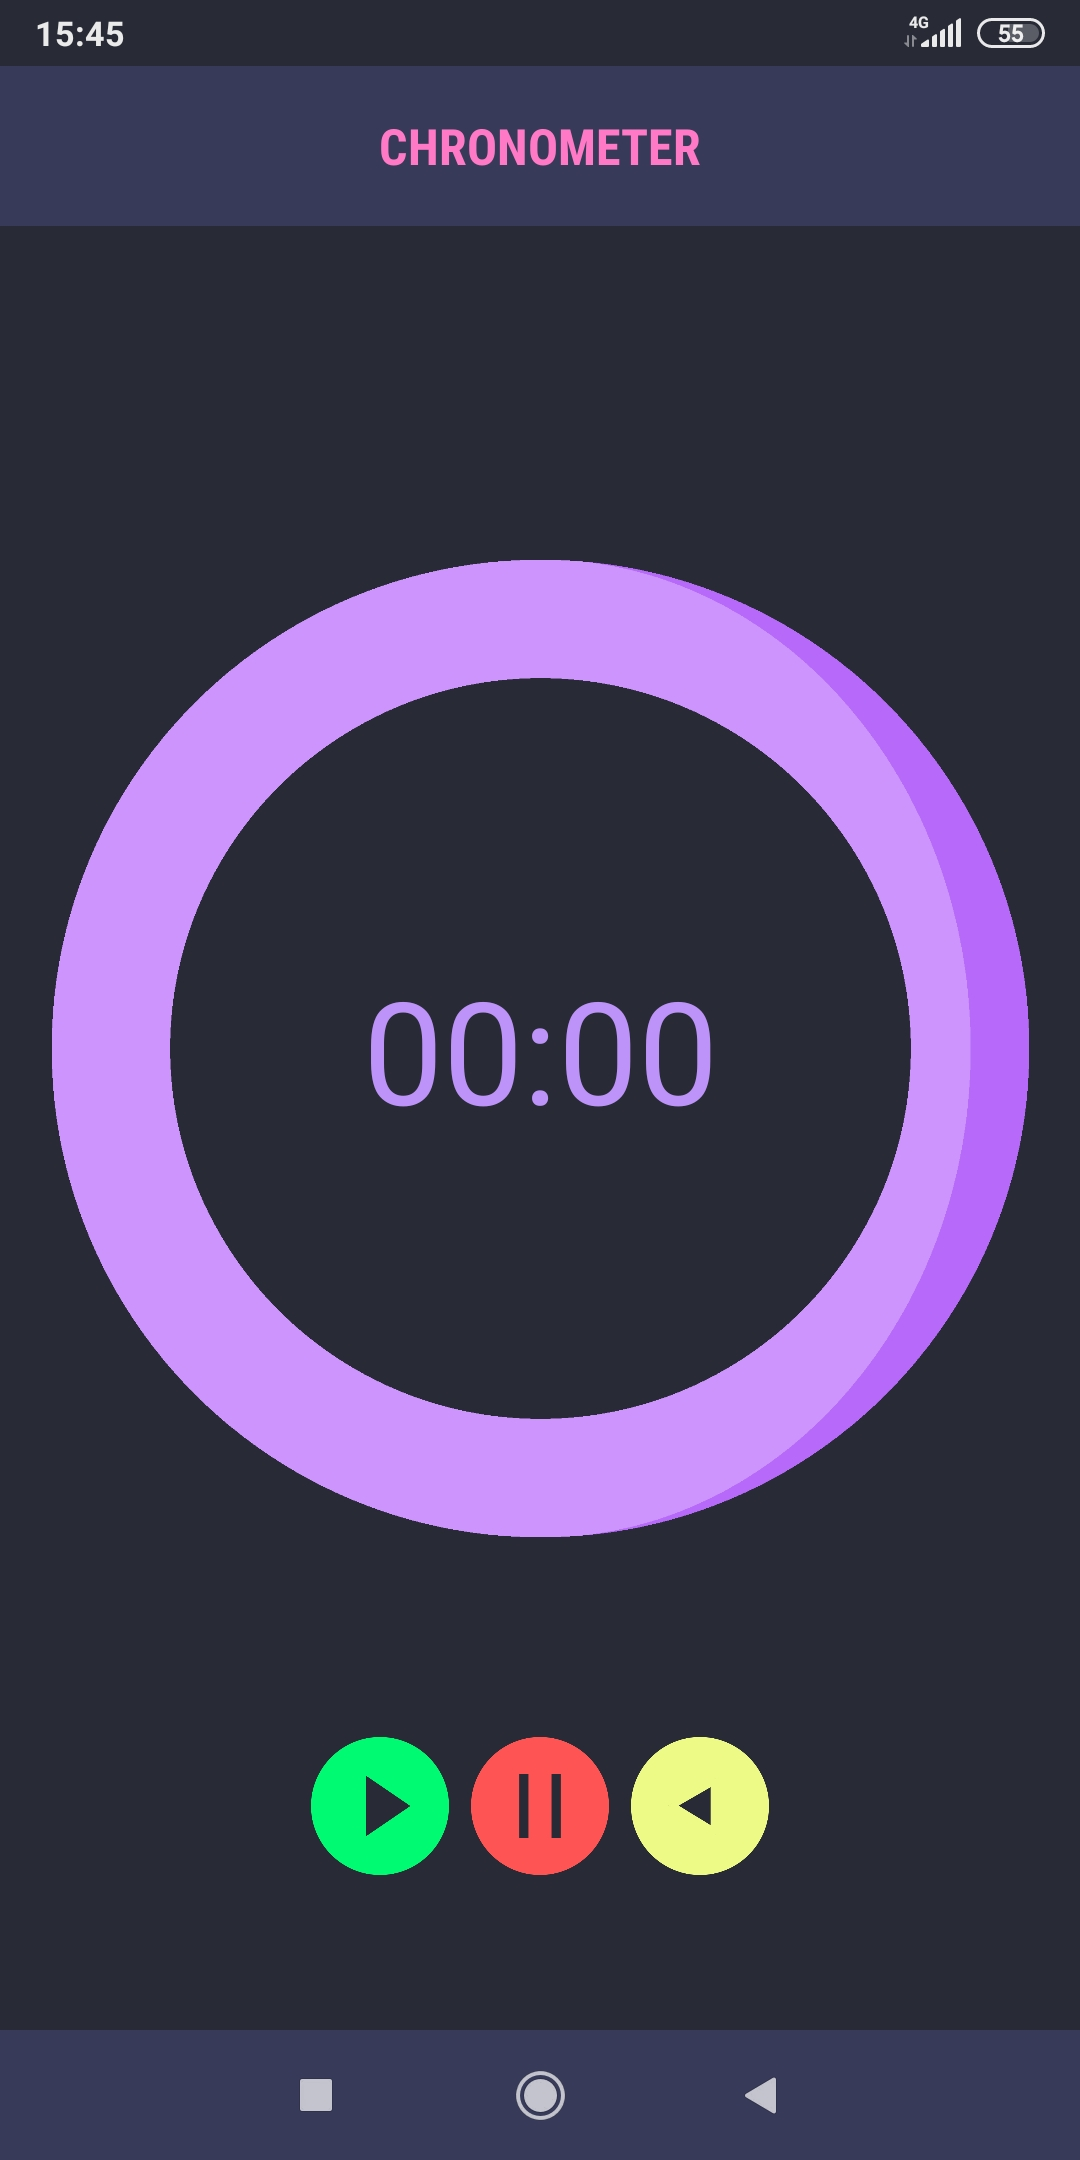
\includegraphics[width=0.5\linewidth]{fig/Capturas de pantalla de la aplicación/chronometer.jpg}
    \caption{Cronometro}
    \label{fig:cronometro}
\end{figure}

\subsection{Registro de puntos durante partidas}

En la última utilidad que se ha implementado podremos seleccionar un número de jugadores, comprendido entre 1 a 30 jugadores, el cual permitirá apuntar los nombres y los puntos de todos los jugadores sin depender de papel y lápiz.

Los nombres se tienen que añadir directamente con el teclado, pero los puntos pueden ser escritos con el teclado o haciendo uso de los botones que tenemos debajo de cada nombre para sumar o restar un punto a la puntuación del jugador.

\begin{figure}[H]
    \centering
    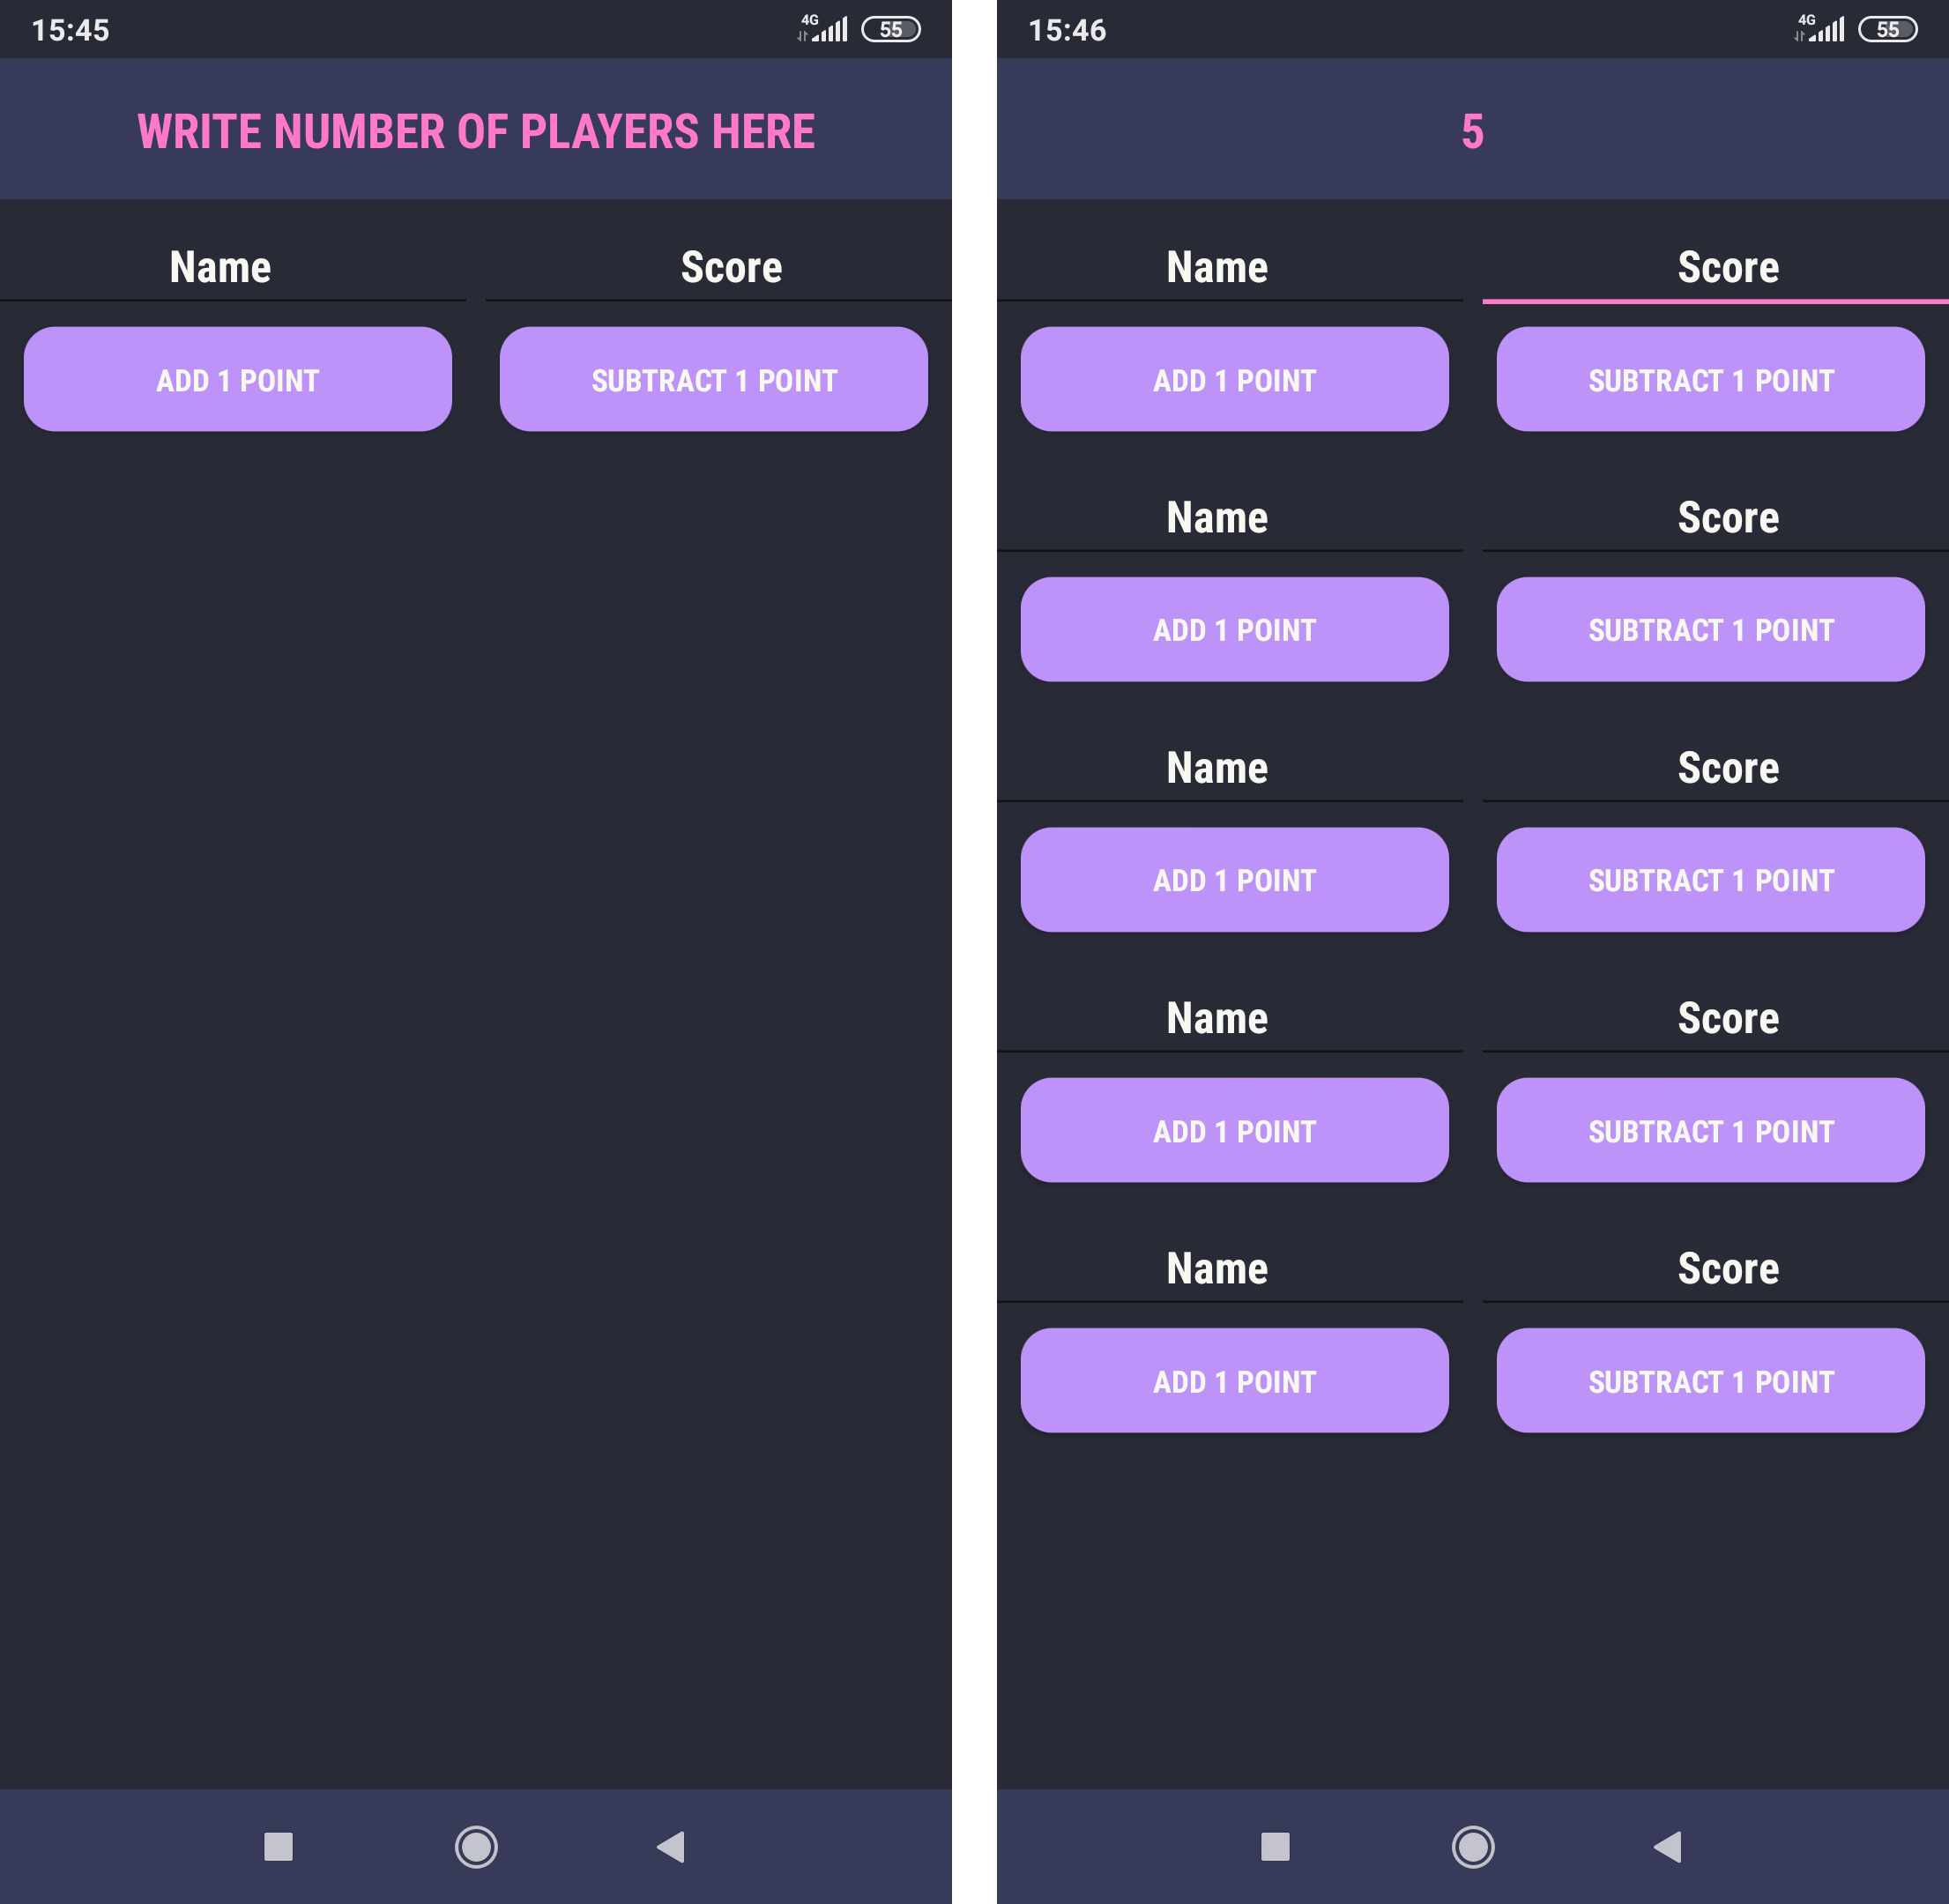
\includegraphics[width=1\linewidth]{fig/Capturas de pantalla de la aplicación/score points.png}
    \caption{Registro de puntos durante partidas}
    \label{fig:registro puntos}
\end{figure}

\newpage